\chapter{Branching and Merging}\label{svn.branchmerge}

\begin{quote}
``君子务本 (It is upon the Trunk that a gentleman works.)''

--- Confucius
\end{quote}

Branching and merging are fundamental aspects of version control, simple
enough to explain conceptually but offering just enough complexity and
nuance to merit their own chapter in this book. Herein,
we\textquotesingle ll introduce you to the general ideas behind these
operations as well as Subversion\textquotesingle s somewhat unique
approach to them. If you\textquotesingle ve not familiarized yourself
with Subversion\textquotesingle s basic concepts (found in
\hyperref[svn.basic]{Fundamental Concepts}), we recommend that you do so
before reading this chapter.

\section{What\textquotesingle s a Branch?}\label{svn.branchmerge.whatis}

Suppose it\textquotesingle s your job to maintain a document for a
division in your company---a handbook of some sort. One day a different
division asks you for the same handbook, but with a few parts
``tweaked'' for them, since they do things slightly differently.

What do you do in this situation? You do the obvious: make a second copy
of your document and begin maintaining the two copies separately. As
each department asks you to make small changes, you incorporate them
into one copy or the other.

You often want to make the same change to both copies. For example, if
you discover a typo in the first copy, it\textquotesingle s very likely
that the same typo exists in the second copy. The two documents are
almost the same, after all; they differ only in small, specific ways.

This is the basic concept of a branch---namely, a line of development
that exists independently of another line, yet still shares a common
history if you look far enough back in time. A branch always begins life
as a copy of something, and moves on from there, generating its own
history (see \hyperref[svn.branchmerge.whatis.dia-1]{Branches of
development}).

\begin{figure}
\centering
\pandocbounded{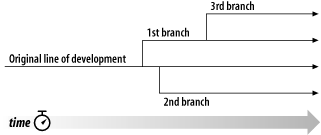
\includegraphics[keepaspectratio]{images/ch04dia1.png}}
\caption{Branches of development}\label{svn.branchmerge.whatis.dia-1}
\end{figure}

Subversion has commands to help you maintain parallel branches of your
files and directories. It allows you to create branches by copying your
data, and remembers that the copies are related to one another. It also
helps you duplicate changes from one branch to another. Finally, it can
make portions of your working copy reflect different branches so that
you can ``mix and match'' different lines of development in your daily
work.

\section{Using Branches}\label{svn.branchmerge.using}

At this point, you should understand how each commit creates a new state
of the filesystem tree (called a ``revision'') in the repository. If you
don\textquotesingle t, go back and read about revisions in
\hyperref[svn.basic.in-action.revs]{Revisions}.

Let\textquotesingle s revisit the example from
\hyperref[svn.basic]{Fundamental Concepts}. Remember that you and your
collaborator, Sally, are sharing a repository that contains two
projects, \texttt{paint} and \texttt{calc}. Notice that in
\hyperref[svn.branchmerge.using.dia-1]{Starting repository layout},
however, each project directory now contains subdirectories named
\texttt{trunk} and \texttt{branches}. The reason for this will soon
become clear.

\begin{figure}
\centering
\pandocbounded{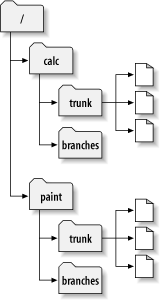
\includegraphics[keepaspectratio]{images/ch04dia2.png}}
\caption{Starting repository layout}\label{svn.branchmerge.using.dia-1}
\end{figure}

As before, assume that Sally and you both have working copies of the
``calc'' project. Specifically, you each have a working copy of
\texttt{/calc/trunk}. All the files for the project are in this
subdirectory rather than in \texttt{/calc} itself, because your team has
decided that \texttt{/calc/trunk} is where the ``main line'' of
development is going to take place.

Let\textquotesingle s say that you\textquotesingle ve been given the
task of implementing a large software feature. It will take a long time
to write, and will affect all the files in the project. The immediate
problem is that you don\textquotesingle t want to interfere with Sally,
who is in the process of fixing small bugs here and there.
She\textquotesingle s depending on the fact that the latest version of
the project (in \texttt{/calc/trunk}) is always usable. If you start
committing your changes bit by bit, you\textquotesingle ll surely break
things for Sally (and other team members as well).

One strategy is to crawl into a hole: you can stop sharing information
for a week or two, gutting and reorganizing all the files in your
private working copy but not committing or updating until
you\textquotesingle re completely finished with your task. There are a
number of problems with this, though. First, it\textquotesingle s not
very safe. Should something bad happen to your working copy or computer,
you risk losing all your changes. Second, it\textquotesingle s not very
flexible. Unless you manually replicate your changes across different
working copies or computers, you\textquotesingle re stuck trying to make
your changes in a single working copy. Similarly, it\textquotesingle s
difficult to share your work-in-progress with anyone else. A common
software development ``best practice'' is to allow your peers to review
your work as you go. If nobody sees your intermediate commits, you lose
potential feedback and may end up going down the wrong path for weeks
before another person on your team notices. Finally, when
you\textquotesingle re finished with all your changes, you might find it
very difficult to merge your completed work with the rest of the
company\textquotesingle s main body of code. Sally (or others) may have
made many other changes in the repository that are difficult to
incorporate into your working copy when you eventually run
\texttt{svn\ update} after weeks of isolation.

The better solution is to create your own branch, or line of
development, in the repository. This allows you to save your
not-yet-completed work frequently without interfering with
others\textquotesingle{} changes and while still selectively sharing
information with your collaborators. You\textquotesingle ll see exactly
how this works as we continue.

\subsection{Creating a Branch}\label{svn.branchmerge.using.create}

Creating a branch is very simple---you make a copy of your project tree
in the repository using the \texttt{svn\ copy} command. Since your
project\textquotesingle s source code is rooted in the
\texttt{/calc/trunk} directory, it\textquotesingle s that directory that
you\textquotesingle ll copy. Where should the new copy live? Wherever
you wish. The repository location in which branches are stashed is left
by Subversion as a matter of project policy. Finally, your branch will
need a name to distinguish it from other branches. Once again, the name
you choose is unimportant to Subversion---you can use whatever name
works best for you and your team.

Let\textquotesingle s assume that your team (like most) has a policy of
creating branches in the \texttt{branches} directory that is a sibling
of the project\textquotesingle s trunk (the \texttt{/calc/branches}
directory in our scenario). Lacking inspiration, you settle on
\texttt{my-calc-branch} as the name you wish to give your branch. This
means that you\textquotesingle ll create a new directory,
\texttt{/calc/branches/my-calc-branch}, which begins its life as a copy
of \texttt{/calc/trunk}.

You may already have seen \texttt{svn\ copy} used to copy one file to
another within a working copy. But it can also be used to do a remote
copy---a copy that immediately results in a newly committed repository
revision and for which no working copy is required at all. Just copy one
URL to another:

\begin{verbatim}
$ svn copy ^/calc/trunk ^/calc/branches/my-calc-branch \
           -m "Creating a private branch of /calc/trunk."

Committed revision 341.
$
\end{verbatim}

This command causes a near-instantaneous commit in the repository,
creating a new directory in revision 341. The new directory is a copy of
\texttt{/calc/trunk}. This is shown in
\hyperref[svn.branchmerge.using.create.dia-1]{Repository with new
copy}.\footnote{Subversion does not support copying between different
  repositories. When using URLs with \texttt{svn\ copy} or
  \texttt{svn\ move}, you can only copy items within the same
  repository.} While it\textquotesingle s also possible to create a
branch by using \texttt{svn\ copy} to duplicate a directory within the
working copy, this technique isn\textquotesingle t recommended. It can
be quite slow, in fact! Copying a directory on the client side is a
linear-time operation, in that it actually has to duplicate every file
and subdirectory within that working copy directory on the local disk.
Copying a directory on the server, however, is a constant-time
operation, and it\textquotesingle s the way most people create branches.
In addition, this practice raises the possibility of copying
mixed-revision working copies. This isn\textquotesingle t inherently
dangerous, but can cause unnecessary complications later during merging.
If you do choose to create a branch by copying a working copy path, you
should be sure the source directory has no local modifications and is
not at mixed-revisions.

\begin{figure}
\centering
\pandocbounded{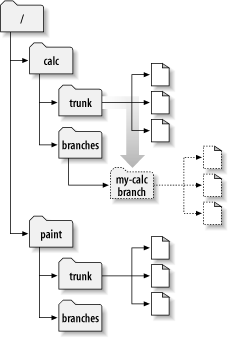
\includegraphics[keepaspectratio]{images/ch04dia3.png}}
\caption{Repository with new
copy}\label{svn.branchmerge.using.create.dia-1}
\end{figure}

Cheap Copies

Subversion\textquotesingle s repository has a special design. When you
copy a directory, you don\textquotesingle t need to worry about the
repository growing huge---Subversion doesn\textquotesingle t actually
duplicate any data. Instead, it creates a new directory entry that
points to an \emph{existing} tree. If you\textquotesingle re an
experienced Unix user, you\textquotesingle ll recognize this as the same
concept behind a hard link. As further changes are made to files and
directories beneath the copied directory, Subversion continues to employ
this hard link concept where it can. It duplicates data only when it is
necessary to disambiguate different versions of objects.

This is why you\textquotesingle ll often hear Subversion users talk
about ``cheap copies.'' It doesn\textquotesingle t matter how large the
directory is---it takes a very tiny, constant amount of time and space
to make a copy of it. In fact, this feature is the basis of how commits
work in Subversion: each revision is a ``cheap copy'' of the previous
revision, with a few items lazily changed within. (To read more about
this, visit Subversion\textquotesingle s web site and read about the
``bubble up'' method in Subversion\textquotesingle s design documents.)

Of course, these internal mechanics of copying and sharing data are
hidden from the user, who simply sees copies of trees. The main point
here is that copies are cheap, both in time and in space. If you create
a branch entirely within the repository (by running
\texttt{svn\ copy\ URL1\ URL2}), it\textquotesingle s a quick,
constant-time operation. Make branches as often as you want.

\subsection{Working with Your Branch}\label{svn.branchmerge.using.work}

Now that you\textquotesingle ve created a branch of the project, you can
check out a new working copy to start using it:

\begin{verbatim}
$ svn checkout http://svn.example.com/repos/calc/branches/my-calc-branch
A    my-calc-branch/doc
A    my-calc-branch/src
A    my-calc-branch/doc/INSTALL
A    my-calc-branch/src/real.c
A    my-calc-branch/src/main.c
A    my-calc-branch/src/button.c
A    my-calc-branch/src/integer.c
A    my-calc-branch/Makefile
A    my-calc-branch/README
Checked out revision 341.

$
\end{verbatim}

There\textquotesingle s nothing special about this working copy; it
simply mirrors a different directory in the repository. When you commit
changes, however, Sally won\textquotesingle t see them when she updates,
because her working copy is of \texttt{/calc/trunk}. (Be sure to read
\hyperref[svn.branchmerge.switchwc]{Traversing Branches} later in this
chapter: the \texttt{svn\ switch} command is an alternative way of
creating a working copy of a branch.)

Let\textquotesingle s pretend that a week goes by, and the following
commits happen:

\begin{itemize}
\item
  You make a change to
  \texttt{/calc/branches/my-calc-branch/src/button.c}, which creates
  revision 342.
\item
  You make a change to
  \texttt{/calc/branches/my-calc-branch/src/integer.c}, which creates
  revision 343.
\item
  Sally makes a change to \texttt{/calc/trunk/src/integer.c}, which
  creates revision 344.
\end{itemize}

Now two independent lines of development (shown in
\hyperref[svn.branchmerge.using.work.dia-1]{The branching of one
file\textquotesingle s history}) are happening on \texttt{integer.c}.

\begin{figure}
\centering
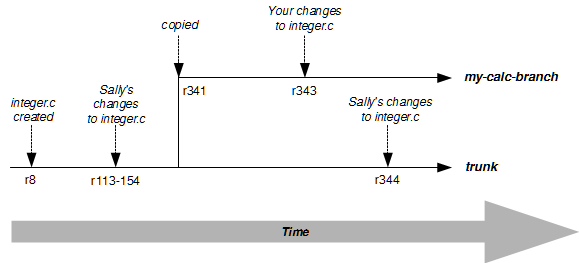
\includegraphics[width=4.81in,height=2.18in]{images/basic-branch.png}
\caption{The branching of one file\textquotesingle s
history}\label{svn.branchmerge.using.work.dia-1}
\end{figure}

Things get interesting when you look at the history of changes made to
your copy of \texttt{integer.c}:

\begin{verbatim}
$ pwd
/home/user/my-calc-branch

$ svn log -v src/integer.c
------------------------------------------------------------------------
r343 | user | 2013-02-15 14:11:09 -0500 (Fri, 15 Feb 2013) | 1 line
Changed paths:
   M /calc/branches/my-calc-branch/src/integer.c

* integer.c:  frozzled the wazjub.
------------------------------------------------------------------------
r341 | user | 2013-02-15 07:41:25 -0500 (Fri, 15 Feb 2013) | 1 line
Changed paths:
   A /calc/branches/my-calc-branch (from /calc/trunk:340)

Creating a private branch of /calc/trunk.
------------------------------------------------------------------------
r154 | sally | 2013-01-30 04:20:03 -0500 (Wed, 30 Jan 2013) | 2 lines
Changed paths:
   M /calc/trunk/src/integer.c

* integer.c:  changed a docstring.
------------------------------------------------------------------------
…
------------------------------------------------------------------------
r113 | sally | 2013-01-26 15:50:21 -0500 (Sat, 26 Jan 2013) | 2 lines
Changed paths:
   M /calc/trunk/src/integer.c

* integer.c: Revise the fooplus API.
------------------------------------------------------------------------
r8 | sally | 2013-01-17 16:55:36 -0500 (Thu, 17 Jan 2013) | 1 line
Changed paths:
   A /calc/trunk/Makefile
   A /calc/trunk/README
   A /calc/trunk/doc/INSTALL
   A /calc/trunk/src/button.c
   A /calc/trunk/src/integer.c
   A /calc/trunk/src/main.c
   A /calc/trunk/src/real.c

Initial trunk code import for calc project.
------------------------------------------------------------------------
\end{verbatim}

Notice that Subversion is tracing the history of your
branch\textquotesingle s \texttt{integer.c} all the way back through
time, even traversing the point where it was copied. It shows the
creation of the branch as an event in the history, because
\texttt{integer.c} was implicitly copied when all of
\texttt{/calc/trunk/} was copied. Now look at what happens when Sally
runs the same command on her copy of the file:

\begin{verbatim}
$ pwd
/home/sally/calc

$ svn log -v src/integer.c
------------------------------------------------------------------------
r344 | sally | 2013-02-15 16:44:44 -0500 (Fri, 15 Feb 2013) | 1 line
Changed paths:
   M /calc/trunk/src/integer.c

Refactor the bazzle functions.
------------------------------------------------------------------------
r154 | sally | 2013-01-30 04:20:03 -0500 (Wed, 30 Jan 2013) | 2 lines
Changed paths:
   M /calc/trunk/src/integer.c

* integer.c:  changed a docstring.
------------------------------------------------------------------------
…
------------------------------------------------------------------------
r113 | sally | 2013-01-26 15:50:21 -0500 (Sat, 26 Jan 2013) | 2 lines
Changed paths:
   M /calc/trunk/src/integer.c

* integer.c: Revise the fooplus API.
------------------------------------------------------------------------
r8 | sally | 2013-01-17 16:55:36 -0500 (Thu, 17 Jan 2013) | 1 line
Changed paths:
   A /calc/trunk/Makefile
   A /calc/trunk/README
   A /calc/trunk/doc/INSTALL
   A /calc/trunk/src/button.c
   A /calc/trunk/src/integer.c
   A /calc/trunk/src/main.c
   A /calc/trunk/src/real.c

Initial trunk code import for calc project.
------------------------------------------------------------------------
\end{verbatim}

Sally sees her own revision 344 change, but not the change you made in
revision 343. As far as Subversion is concerned, these two commits
affected different files in different repository locations. However,
Subversion \emph{does} show that the two files share a common history.
Before the branch copy was made in revision 341, the files used to be
the same file. That\textquotesingle s why you and Sally both see the
changes made between revisions 8 and 154.

\subsection{The Key Concepts Behind
Branching}\label{svn.branchmerge.using.concepts}

You should remember two important lessons from this section. First,
Subversion has no internal concept of a branch---it knows only how to
make copies. When you copy a directory, the resultant directory is only
a ``branch'' because \emph{you} attach that meaning to it. You may think
of the directory differently, or treat it differently, but to Subversion
it\textquotesingle s just an ordinary directory that happens to carry
some extra historical information.

Second, because of this copy mechanism, Subversion\textquotesingle s
branches exist as \emph{normal filesystem directories} in the
repository. This is different from other version control systems, where
branches are typically defined by adding extra-dimensional ``labels'' to
collections of files. The location of your branch directory
doesn\textquotesingle t matter to Subversion. Most teams follow a
convention of putting all branches into a \texttt{/branches} directory,
but you\textquotesingle re free to invent any policy you wish.

\section{Basic Merging}\label{svn.branchmerge.basicmerging}

Now you and Sally are working on parallel branches of the project:
you\textquotesingle re working on a private branch, and Sally is working
on the trunk, or main line of development.

For projects that have a large number of contributors,
it\textquotesingle s common for most people to have working copies of
the trunk. Whenever someone needs to make a long-running change that is
likely to disrupt the trunk, a standard procedure is to create a private
branch and commit changes there until all the work is complete.

So, the good news is that you and Sally aren\textquotesingle t
interfering with each other. The bad news is that it\textquotesingle s
very easy to drift \emph{too} far apart. Remember that one of the
problems with the ``crawl in a hole'' strategy is that by the time
you\textquotesingle re finished with your branch, it may be
near-impossible to merge your changes back into the trunk without a huge
number of conflicts.

Instead, you and Sally might continue to share changes as you work.
It\textquotesingle s up to you to decide which changes are worth
sharing; Subversion gives you the ability to selectively ``copy''
changes between branches. And when you\textquotesingle re completely
finished with your branch, your entire set of branch changes can be
copied back into the trunk. In Subversion terminology, the general act
of replicating changes from one branch to another is called merging, and
it is performed using various invocations of the \texttt{svn\ merge}
subcommand.

In the examples that follow, we\textquotesingle re assuming that both
your Subversion client and server are running Subversion 1.8 (or later).
If either client or server is older than version 1.5, things are more
complicated: the system won\textquotesingle t track changes
automatically, forcing you to use painful manual methods to achieve
similar results. That is, you\textquotesingle ll always need to use the
detailed merge syntax to specify specific ranges of revisions to
replicate (see \hyperref[svn.branchmerge.advanced.advancedsyntax]{Merge
Syntax: Full Disclosure} later in this chapter), and take special care
to keep track of what\textquotesingle s already been merged and what
hasn\textquotesingle t. For this reason, we \emph{strongly} recommend
that you make sure your client and server are at least at version 1.5.

\protect\phantomsection\label{svn.branchmerge.basicmerging.mergetracking}
Merge Tracking

Subversion 1.5 introduced the merge tracking feature to Subversion.
Prior to this feature keeping track of merges required cumbersome manual
procedures or the use of external tools. Subsequent releases of
Subversion introduced many enhancements and bug fixes to merge tracking,
which is why we recommend using the most recent versions for both your
server and client. Keep in mind that even if your server is running
1.5-1.7, you can still use a 1.8 client. This is particularly important
with regard to merge tracking, because the overwhelming majority of
fixes and enhancements to it are on the client side.

\subsection{Changesets}\label{svn.branchmerge.changesets}

Before we proceed further, we should warn you that
there\textquotesingle s a lot of discussion of ``changes'' in the pages
ahead. A lot of people experienced with version control systems use the
terms ``change'' and ``changeset'' interchangeably, and we should
clarify what Subversion understands as a changeset.

Everyone seems to have a slightly different definition of changeset, or
at least a different expectation of what it means for a version control
system to have one. For our purposes, let\textquotesingle s say that a
changeset is just a collection of changes with a unique name. The
changes might include textual edits to file contents, modifications to
tree structure, or tweaks to metadata. In more common speak, a changeset
is just a patch with a name you can refer to.

In Subversion, a global revision number \textless N\textgreater{} names
a tree in the repository: it\textquotesingle s the way the repository
looked after the \textless N\textgreater th commit. It\textquotesingle s
also the name of an implicit changeset: if you compare tree
\textless N\textgreater{} with tree \textless N\textgreater-1, you can
derive the exact patch that was committed. For this reason,
it\textquotesingle s easy to think of revision \textless N\textgreater{}
as not just a tree, but a changeset as well. If you use an issue tracker
to manage bugs, you can use the revision numbers to refer to particular
patches that fix bugs---for example, ``this issue was fixed by r9238.''
Somebody can then run \texttt{svn\ log\ -r\ 9238} to read about the
exact changeset that fixed the bug, and run \texttt{svn\ diff\ -c\ 9238}
to see the patch itself. And (as you\textquotesingle ll see shortly)
Subversion\textquotesingle s \texttt{svn\ merge} command is able to use
revision numbers. You can merge specific changesets from one branch to
another by naming them in the merge arguments: passing \texttt{-c\ 9238}
to \texttt{svn\ merge} would merge changeset r9238 into your working
copy.

\subsection{Keeping a Branch in
Sync}\label{svn.branchmerge.basicmerging.stayinsync}

Continuing with our running example, let\textquotesingle s suppose that
a week has passed since you started working on your private branch. Your
new feature isn\textquotesingle t finished yet, but at the same time you
know that other people on your team continue to make important changes
in the project\textquotesingle s \texttt{/trunk}. It\textquotesingle s
in your best interest to replicate those changes to your own branch,
just to make sure they mesh well with your changes. This is done by
performing an automatic sync merge---a merge operation designed to bring
your branch up to date with any changes made to its ancestral parent
branch since your branch was created. An ``automatic'' merge is simply
one in which you provide the bare minimum of information required for a
merge (i.e. a single merge source and a working copy target) and let
Subversion determine which changes need merging---no changesets are
passed to \texttt{svn\ merge} via the \texttt{-r} or \texttt{-c} options
in an automatic merge.

Frequently keeping your branch in sync with the main development line
helps prevent ``surprise'' conflicts when the time comes for you to fold
your changes back into the trunk.

Subversion is aware of the history of your branch and knows when it
split away from the trunk. To perform a sync merge, first make sure your
working copy of the branch is ``clean''---that it has no local
modifications reported by \texttt{svn\ status}. Then simply run:

\begin{verbatim}
$ pwd
/home/user/my-calc-branch

$ svn merge ^/calc/trunk
--- Merging r341 through r351 into '.':
U    doc/INSTALL
U    src/real.c
U    src/button.c
U    Makefile
--- Recording mergeinfo for merge of r341 through r351 into '.':
 U   .
 $
\end{verbatim}

This basic syntax---\texttt{svn\ merge\ URL}---tells Subversion to merge
all changes which have not been previously merged from the URL to the
current working directory (which is typically the root of your working
copy). Notice that we\textquotesingle re using the caret (\texttt{\^{}})
syntax\footnote{This was introduced in svn 1.6.} to avoid having to type
out the entire \texttt{/trunk} URL. Also note the ``Recording mergeinfo
for merge\ldots{}'' notification. This tells you that the merge is
updating the \texttt{svn:mergeinfo} property. We\textquotesingle ll
discuss both this property and these notifications later in this
chapter, in \hyperref[svn.branchmerge.basicmerging.mergeinfo]{Mergeinfo
and Previews}.

In this book and elsewhere (Subversion mailing lists, articles on merge
tracking, etc.) you will frequently come across the term mergeinfo. This
is simply shorthand for the \texttt{svn:mergeinfo} property.

Keeping a Branch in Sync Without Merge Tracking

You may not always be able to use Subversion\textquotesingle s merge
tracking feature, perhaps because your server is running Subversion 1.4
or earlier or you must use an older client. In such a scenario, you can
of course still perform merges, but Subversion will need you to manually
do many of the historical calculations that it automatically does on
your behalf when the merge tracking feature is available.

To replicate the most recent trunk changes you need to perform sync
merges the ``old-fashioned'' way---by specifying ranges of revisions you
wish to merge.

Using the ongoing example, you know that you branched
\texttt{/calc/trunk} to \texttt{/calc/branches/my-calc-branch} in
revision 341:

\begin{verbatim}
$ svn log -v -r341
------------------------------------------------------------------------
r341 | user | 2013-02-15 07:41:25 -0500 (Fri, 15 Feb 2013) | 1 line
Changed paths:
   A /calc/branches/my-calc-branch (from /calc/trunk:340)

Creating a private branch of /calc/trunk.
------------------------------------------------------------------------
\end{verbatim}

When you are ready to synchronize your branch with the ongoing changes
from trunk, you specify the starting revision as the revision of
\texttt{/calc/trunk} which the branch was copied from and the ending
revision as the youngest change on \texttt{/calc/trunk}. You can find
the latter with the \texttt{svn\ log} command with the \texttt{-r} set
to \texttt{HEAD}:

\begin{verbatim}
$ svn log -q -rHEAD http://svn.example.com/repos/calc/trunk
------------------------------------------------------------------------
r351 | sally | 2013-02-16 08:04:22 -0500 (Sat, 16 Feb 2013)
------------------------------------------------------------------------

$ svn merge http://svn.example.com/repos/calc/trunk -r340:351
U    doc/INSTALL
U    src/real.c
U    src/button.c
U    Makefile
\end{verbatim}

After any conflicts have been resolved, you can commit the merged
changes to your branch. Now, to avoid accidentally trying to merge these
same changes into your branch again in the future,
you\textquotesingle ll need to record the fact that
you\textquotesingle ve already merged them. But where should that record
be kept? One of the simplest places to record this information is in the
log message for the commit of the merge:

\begin{verbatim}
$ svn ci -m "Sync the my-calc-branch with ^/calc/trunk through r351."
…
\end{verbatim}

The next time you sync \texttt{/calc/branches/my-calc-branch} with
\texttt{/calc/trunk} you repeat this process, except that the starting
revision is the \emph{youngest} revision that\textquotesingle s already
been merged in from the trunk. If you\textquotesingle ve been keeping
good records of your merges in the commit log messages, you should be
able to determine what that youngest revision was by reading the
revision logs associated with your branch. Once you know your starting
revision, you can perform another sync merge:

\begin{verbatim}
$ svn log -q -rHEAD http://svn.example.com/repos/calc/trunk
------------------------------------------------------------------------
r959 | sally | 2013-03-5 7:30:21 -0500 (Tue, 05 Mar 2013)
------------------------------------------------------------------------

$ svn merge http://svn.example.com/repos/calc/trunk -r351:959
…
\end{verbatim}

After running the prior example, your branch working copy now contains
new local modifications, and these edits are duplications of all of the
changes that have happened on the trunk since you first created your
branch:

\begin{verbatim}
$ svn status
 M      .
M       Makefile
M       doc/INSTALL
M       src/button.c
M       src/real.c
\end{verbatim}

At this point, the wise thing to do is look at the changes carefully
with \texttt{svn\ diff}, and then build and test your branch. Notice
that the current working directory (``\texttt{.}'') has also been
modified; \texttt{svn\ diff} shows that its \texttt{svn:mergeinfo}
property has been created.

\begin{verbatim}
$ svn diff --depth empty .
Index: .
===================================================================
--- .   (revision 351)
+++ .   (working copy)

Property changes on: .
___________________________________________________________________
Added: svn:mergeinfo
   Merged /calc/trunk:r341-351
\end{verbatim}

This new property is important merge-related metadata that you should
\emph{not} touch, since it is needed by future \texttt{svn\ merge}
commands. (We\textquotesingle ll learn more about this metadata later in
the chapter.)

After performing the merge, you might also need to resolve some
conflicts---just as you do with \texttt{svn\ update}---or possibly make
some small edits to get things working properly. (Remember, just because
there are no \emph{syntactic} conflicts doesn\textquotesingle t mean
there aren\textquotesingle t any \emph{semantic} conflicts!) If you
encounter serious problems, you can always abort the local changes by
running \texttt{svn\ revert\ .\ -R} (which will undo all local
modifications) and starting a long ``what\textquotesingle s going on?''
discussion with your collaborators. If things look good, however, you
can submit these changes into the repository:

\begin{verbatim}
$ svn commit -m "Sync latest trunk changes to my-calc-branch."
Sending        .
Sending        Makefile
Sending        doc/INSTALL
Sending        src/button.c
Sending        src/real.c
Transmitting file data ....
Committed revision 352.
\end{verbatim}

At this point, your private branch is now ``in sync'' with the trunk, so
you can rest easier knowing that as you continue to work in isolation,
you\textquotesingle re not drifting too far away from what everyone else
is doing.

Why Not Use Patches Instead?

A question may be on your mind, especially if you\textquotesingle re a
Unix user: why bother to use \texttt{svn\ merge} at all? Why not simply
use \texttt{svn\ patch} or the operating system\textquotesingle s
\texttt{patch} command to accomplish the same job? For example:

\begin{verbatim}
$ cd my-calc-branch

$ svn diff -r 341:351 ^/calc/trunk > my-patch-file

$ svn patch my-patch-file
U         doc/INSTALL
U         src/real.c
U         src/button.c
U         Makefile
\end{verbatim}

In this particular example, there really isn\textquotesingle t much
difference. But \texttt{svn\ merge} has special abilities that surpass
the \texttt{patch} program. The file format used by \texttt{patch} is
quite limited; it\textquotesingle s able to tweak file contents only.
There\textquotesingle s no way to represent changes to \emph{trees},
such as the addition, removal, or renaming of files and directories. Nor
can the \texttt{patch} program notice changes to properties. If
Sally\textquotesingle s change had, say, added a new directory, the
output of \texttt{svn\ diff} wouldn\textquotesingle t have mentioned it
at all. \texttt{svn\ diff} outputs only the limited patch format, so
there are some ideas it simply can\textquotesingle t express. Even
Subversion\textquotesingle s own \texttt{svn\ patch} subcommand, while
more flexible than the \texttt{patch} program, still has similar
limitations.

The \texttt{svn\ merge} command, however, can express changes in tree
structure and properties by directly applying them to your working copy.
Even more important, this command records the changes that have been
duplicated to your branch so that Subversion is aware of exactly which
changes exist in each location (see
\hyperref[svn.branchmerge.basicmerging.mergeinfo]{Mergeinfo and
Previews}). This is a critical feature that makes branch management
usable; without it, users would have to manually keep notes on which
sets of changes have or haven\textquotesingle t been merged yet.

Suppose that another week has passed. You\textquotesingle ve committed
more changes to your branch, and your comrades have continued to improve
the trunk as well. Once again, you want to replicate the latest trunk
changes to your branch and bring yourself in sync. Just run the same
merge command again!

\begin{verbatim}
$ svn merge ^/calc/trunk
svn: E195020: Cannot merge into mixed-revision working copy [352:357]; try up\
dating first
$
\end{verbatim}

Well that was unexpected! After making changes to your branch over the
past week you now find yourself with a working copy that contains a
mixture of revisions (see
\hyperref[svn.basic.in-action.mixedrevs]{Mixed-revision working
copies}). With Subversion 1.7 and later, the \texttt{svn\ merge}
subcommand disables merges into mixed-revision working copies by
default. Without going into too much detail, this is because of
limitations in the way merges are tracked by the \texttt{svn:mergeinfo}
property (see
\hyperref[svn.branchmerge.basicmerging.mergeinfo]{Mergeinfo and
Previews} for details). These limitations mean that merges into
mixed-revision working copies can result in unexpected text and tree
conflicts.\footnote{The \texttt{svn\ merge} subcommand option
  \texttt{-\/-allow-mixed-revisions} allows you to override this
  prohibition, but you should only do so if you understand the
  ramifications and have a good reason for it.} We don\textquotesingle t
want any needless conflicts, so we update the working copy and then
reattempt the merge.

\begin{verbatim}
$ svn up
Updating '.':
At revision 361.

$ svn merge ^/calc/trunk
--- Merging r352 through r361 into '.':
U    src/real.c
U    src/main.c
--- Recording mergeinfo for merge of r352 through r361 into '.':
 U   .
\end{verbatim}

Subversion knows which trunk changes you previously replicated to your
branch, so it carefully replicates only those changes you
don\textquotesingle t yet have. And once again, you build, test, and
\texttt{svn\ commit} the local modifications to your branch.

\subsection{Subtree Merges and Subtree
Mergeinfo}\label{svn.branchmerge.basicmerging.stayinsync.subtree}

In most of the examples in this chapter the merge target is the root
directory of a branch (see
\hyperref[svn.branchmerge.whatis]{What\textquotesingle s a Branch?}).
While this is a best practice, you may occasionally need to merge
directly to some child of the branch root. This type of merge is called
a subtree merge and the mergeinfo recorded to describe it is called
subtree mergeinfo. There is nothing special about subtree merges or
subtree mergeinfo. In fact there is really only one important point to
keep in mind about these concepts: the complete record of merges to a
branch may not be contained solely in the mergeinfo on the branch root.
You may have to consider subtree mergeinfo to get a full accounting.
Fortunately Subversion does this for you and rarely will you need to
concern yourself with it. A brief example will help explain:

\begin{verbatim}
# We need to merge r958 from trunk to branches/proj-X/doc/INSTALL,
# but that revision also affects main.c, which we don't want to merge:
$ svn log --verbose --quiet -r 958 ^/
------------------------------------------------------------------------
r958 | bruce | 2011-10-20 13:28:11 -0400 (Thu, 20 Oct 2011)
Changed paths:
   M /trunk/doc/INSTALL
   M /trunk/src/main.c
------------------------------------------------------------------------

# No problem, we'll do a subtree merge targeting the INSTALL file
# directly, but first take a note of what mergeinfo exists on the
# root of the branch:
$ cd branches/proj-X

$ svn propget svn:mergeinfo --recursive
Properties on '.':
  svn:mergeinfo
    /trunk:651-652

# Now we perform the subtree merge, note that merge source
# and target both point to INSTALL:
$ svn merge ^/trunk/doc/INSTALL doc/INSTALL -c 958
--- Merging r958 into 'doc/INSTALL':
U    doc/INSTALL
--- Recording mergeinfo for merge of r958 into 'doc/INSTALL':
 G   doc/INSTALL

# Once the merge is complete there is now subtree mergeinfo on INSTALL:
$ svn propget svn:mergeinfo --recursive
Properties on '.':
  svn:mergeinfo
    /trunk:651-652
Properties on 'doc/INSTALL':
  svn:mergeinfo
    /trunk/doc/INSTALL:651-652,958

# What if we then decide we do want all of r958? Easy, all we need do is
# repeat the merge of that revision, but this time to the root of the
# branch, Subversion notices the subtree mergeinfo on INSTALL and doesn't
# try to merge any changes to it, only the changes to main.c are merged:
$ svn merge ^/subversion/trunk . -c 958
--- Merging r958 into '.':
U    src/main.c
--- Recording mergeinfo for merge of r958 into '.':
 U   .
--- Eliding mergeinfo from 'doc/INSTALL':
 U   doc/INSTALL
\end{verbatim}

You might be wondering why \texttt{INSTALL} in the above example has
mergeinfo for r651-652, when we only merged r958. This is due to
mergeinfo inheritance, which we\textquotesingle ll cover in the sidebar
\hyperref[svn.branchmerge.basicmerging.mergeinfo.inheritance]{Mergeinfo
Inheritance}. Also note that the subtree mergeinfo on
\texttt{doc/INSTALL} was removed, or ``elided''. This is called
mergeinfo elision and it occurs whenever Subversion detects redundant
subtree mergeinfo.

Prior to Subversion 1.7, merges unconditionally updated \emph{all} of
the subtree mergeinfo under the target to describe the merge. For users
with a lot of subtree mergeinfo this meant that relatively ``simple''
merges (e.g. one which applied a diff to only a single file) resulted in
changes to every subtree with mergeinfo, even those that were not
parents of the affected path(s). This caused some level of confusion and
frustration. Subversion 1.7 and later addresses this problem by only
updating the mergeinfo on subtrees which are parents of the paths
modified by the merge (i.e. paths changed, added, or deleted by
application of the difference, see
\hyperref[svn.branchmerge.advanced.advancedsyntax]{Merge Syntax: Full
Disclosure}). The one exception to this behavior regards the actual
merge target; the merge target\textquotesingle s mergeinfo is always
updated to describe the merge, even if the applied difference made no
changes.

\subsection{Reintegrating a
Branch}\label{svn.branchmerge.basicmerging.reintegrate}

What happens when you finally finish your work, though? Your new feature
is done, and you\textquotesingle re ready to merge your branch changes
back to the trunk (so your team can enjoy the bounty of your labor). The
process is simple. First, bring your branch into sync with the trunk
again, just as you\textquotesingle ve been doing all along\footnote{Since
  Subversion 1.7 you don\textquotesingle t absolutely have to do all
  your sync merges to the root of your branch as we do in this example.
  \emph{If} your branch is effectively synced via a series of subtree
  merges then the reintegrate will work, but ask yourself, if the branch
  is effectively synced, then why are you doing subtree merges? Doing so
  is almost always needlessly complex.}:

\begin{verbatim}
$ svn up # (make sure the working copy is up to date)
Updating '.':
At revision 378.

$ svn merge ^/calc/trunk
--- Merging r362 through r378 into '.':
U    src/main.c
--- Recording mergeinfo for merge of r362 through r378 into '.':
 U   .

$ # build, test, ...

$ svn commit -m "Final merge of trunk changes to my-calc-branch."
Sending        .
Sending        src/main.c
Transmitting file data .
Committed revision 379.
\end{verbatim}

Now, use \texttt{svn\ merge} subcommand to automatically replicate your
branch changes back into the trunk. This type of merge is called an
``automatic reintegrate'' merge. You\textquotesingle ll need a working
copy of \texttt{/calc/trunk}. You can get one by doing an
\texttt{svn\ checkout}, dredging up an old trunk working copy from
somewhere on your disk, or using \texttt{svn\ switch} (see
\hyperref[svn.branchmerge.switchwc]{Traversing Branches}).

The term ``reintegrating'' comes from the \texttt{merge} option
\texttt{-\/-reintegrate}. This option is deprecated in Subversion 1.8
(which automatically detects when a reintegrate merge is needed), but is
required for Subversion 1.5 through 1.7 clients when performing
reintegrate merges.

Your trunk working copy cannot have any local edits, switched paths, or
contain a mixture of revisions (see
\hyperref[svn.basic.in-action.mixedrevs]{Mixed-revision working
copies}). While these are typically best practices for merging anyway,
they are \emph{required} for automatic reintegrate merges.

Once you have a clean working copy of the trunk, you\textquotesingle re
ready to merge your branch back into it:

\begin{verbatim}
$ pwd
/home/user/calc-trunk

$ svn update
Updating '.':
At revision 379.

$ svn merge ^/calc/branches/my-calc-branch
--- Merging differences between repository URLs into '.':
U    src/real.c
U    src/main.c
U    Makefile
--- Recording mergeinfo for merge between repository URLs into '.':
 U   .

$ # build, test, verify, ...

$ svn commit -m "Merge my-calc-branch back into trunk!"
Sending        .
Sending        Makefile
Sending        src/main.c
Sending        src/real.c
Transmitting file data ...
Committed revision 380.
\end{verbatim}

Congratulations, your branch-specific changes have now been merged back
into the main line of development. Notice that the automatic reintegrate
merge did a different sort of work than what you\textquotesingle ve done
up until now. Previously, we were asking \texttt{svn\ merge} to grab the
``next set'' of changes from one line of development (the trunk) and
duplicate them to another (your branch). This is fairly straightforward,
and each time Subversion knows how to pick up where it left off. In our
prior examples, you can see that first it merges the ranges 341:351 from
\texttt{/calc/trunk} to \texttt{/calc/branches/my-calc-branch}; later
on, it continues by merging the next contiguously available range,
351:361. When doing the final sync, it merges the range 361:378.

When merging \texttt{/calc/branches/my-calc-branch} back to the
\texttt{/calc/trunk}, however, the underlying mathematics are quite
different. Your feature branch is now a mishmash of both duplicated
trunk changes and private branch changes, so there\textquotesingle s no
simple contiguous range of revisions to copy over. By using an automatic
merge, you\textquotesingle re asking Subversion to carefully replicate
\emph{only} those changes unique to your branch. (And in fact, it does
this by comparing the latest trunk tree with the latest branch tree: the
resulting difference is exactly your branch changes!)

Keep in mind that the automatic reintegrate merges only support the use
case described above. Because of this narrow focus, in addition to the
requirements previously mentioned (up-to-date working copy \footnote{Automatic
  reintegrate merges are allowed if the target is a shallow checkout
  (see \hyperref[svn.advanced.sparsedirs]{Sparse Directories}) but any
  paths affected by the diff which are ``missing'' due to the sparse
  working copy will be skipped---this is probably \emph{not} what you
  intended!} with no mixed-revisions, switched paths or local changes)
it will not function in combination with most of the other
\texttt{svn\ merge} options. You\textquotesingle ll get an error if you
use any non-global options but these: \texttt{-\/-accept},
\texttt{-\/-dry-run}, \texttt{-\/-diff3-cmd}, \texttt{-\/-extensions},
or \texttt{-\/-quiet}.

Now that your private branch is merged to trunk, you may wish to remove
it from the repository:

\begin{verbatim}
$ svn delete ^/calc/branches/my-calc-branch \
             -m "Remove my-calc-branch, reintegrated with trunk in r381."
…
\end{verbatim}

But wait! Isn\textquotesingle t the history of that branch valuable?
What if somebody wants to audit the evolution of your feature someday
and look at all of your branch changes? No need to worry. Remember that
even though your branch is no longer visible in the
\texttt{/calc/branches} directory, its existence is still an immutable
part of the repository\textquotesingle s history. A simple
\texttt{svn\ log} command on the \texttt{/calc/branches} URL will show
the entire history of your branch. Your branch can even be resurrected
at some point, should you desire (see
\hyperref[svn.branchmerge.basicmerging.resurrect]{Resurrecting Deleted
Items}).

If you choose not to delete your branch after reintegrating it to the
trunk you may continue to perform sync merges from the trunk and then
reintegrate the branch again\footnote{Only Subversion 1.8 supports this
  reuse of a feature branch. Earlier versions require some special
  handling before a feature branch can be reintegrated more than once.
  See the earlier version of this chapter for more information:
  \href{https://svnbook.red-bean.com/en/1.7/svn.branchmerge.basicmerging.html\#svn.branchemerge.basicmerging.reintegrate}{}}.
If you do this, only the changes made on your branch after the first
reintegrate are merged to the trunk.

\subsection{Mergeinfo and
Previews}\label{svn.branchmerge.basicmerging.mergeinfo}

The basic mechanism Subversion uses to track changesets---that is, which
changes have been merged to which branches---is by recording data in
versioned properties. Specifically, merge data is tracked in the
\texttt{svn:mergeinfo} property attached to files and directories. (If
you\textquotesingle re not familiar with Subversion properties, see
\hyperref[svn.advanced.props]{Properties}.)

You can examine the mergeinfo property, just like any other versioned
property:

\begin{verbatim}
$ cd my-calc-branch

$ svn pg svn:mergeinfo -v
Properties on '.':
  svn:mergeinfo
    /calc/trunk:341-378
\end{verbatim}

While it is possible to modify \texttt{svn:mergeinfo} just as you might
any other versioned property, we strongly discourage doing so unless you
\emph{really} know what you\textquotesingle re doing.

The amount of \texttt{svn:mergeinfo} on a single path can get quite
large, as can the output of a \texttt{svn\ propget\ -\/-recursive} or
\texttt{svn\ proplist\ -\/-recursive} when dealing with large amounts of
subtree mergeinfo. See
\hyperref[svn.branchmerge.basicmerging.stayinsync.subtree]{Subtree
Merges and Subtree Mergeinfo} . The formatted output produced by the
\texttt{-\/-verbose} option with either of these subcommands is often
very helpful in these cases.

The \texttt{svn:mergeinfo} property is automatically maintained by
Subversion whenever you run \texttt{svn\ merge}. Its value indicates
which changes made to a given path have been replicated into the
directory in question. In our previous example, the path which is the
source of the merged changes is \texttt{/calc/trunk} and the directory
which has received the changes is
\texttt{/calc/branches/my-calc-branch}. Earlier versions of Subversion
maintained the \texttt{svn:mergeinfo} property silently. You could still
detect the changes, after a merge completed, with the \texttt{svn\ diff}
or \texttt{svn\ status} subcommands, but the merge itself gave no
indication when it changed the \texttt{svn:mergeinfo} property. In
Subversion 1.7 and later this is no longer true as there are several
notifications to alert you when a merge updates the
\texttt{svn:mergeinfo} property. These notifications all begin with
``-\/-\/- Recording mergeinfo for'' and appear at the end of the merge.
Unlike other merge notifications, these don\textquotesingle t describe
the application of a difference to a working copy (see
\hyperref[svn.branchmerge.advanced.advancedsyntax]{Merge Syntax: Full
Disclosure}), but instead describe "housekeeping" changes made to keep
track of what was merged.

Subversion also provides a subcommand, \texttt{svn\ mergeinfo}, which is
helpful in seeing the merge relationships between two branches;
specifically which changesets a directory has absorbed or which
changesets it\textquotesingle s still eligible to receive. The latter
gives a sort of preview of which changes a subsequent
\texttt{svn\ merge} operation would replicate to your branch. By
default, \texttt{svn\ mergeinfo} gives an graphical overview of the
relationship between to branches. Returning to our earlier example, we
use the subcommand to analyze the relationship between
\texttt{/calc/trunk} and \texttt{/calc/branches/my-calc-branch}:

\begin{verbatim}
$ cd my-calc-branch

$ svn mergeinfo ^/calc/trunk
    youngest common ancestor
    |         last full merge
    |         |        tip of branch
    |         |        |         repository path

    340                382
    |                  |
  -------| |------------         calc/trunk
     \          /
      \        /
       --| |------------         calc/branches/my-calc-branch
              |        |
              379      382
\end{verbatim}

The diagram shows that \texttt{/calc/branches/my-calc-branch} was copied
from \texttt{/calc/trunk@340} and that most recent automatic merge was
the reintegrate merge we made from the branch to the trunk in r380.
Notice that the diagram does \emph{not} show the four automatic sync
merges we made in revisions 352, 362, 372, and 379. Only the most recent
automatic merge, in either direction\footnote{By ``direction'' we mean
  either trunk-to-branch (automatic sync) or branch-to-trunk (automatic
  reintegrate) merges.}, is shown. This default output is useful for
obtaining an overview of the merges between two branches, but to see the
specific revisions which were merged we use the
\texttt{-\/-show-revs=merged} option:

\begin{verbatim}
$ svn mergeinfo ^/calc/trunk --show-revs merged
r344
r345
r346
…
r366
r367
r368
\end{verbatim}

Likewise, to see which changes are eligible to merge from the trunk to
the branch we can use the \texttt{-\/-show-revs=eligible} option:

\begin{verbatim}
$ svn mergeinfo ^/calc/trunk --show-revs eligible
r380
r381
r382
\end{verbatim}

\protect\phantomsection\label{svn.branchmerge.basicmerging.mergeinfo.operativerevs}
Operative and Inoperative Merge Revisions

The revision lists produced by the \texttt{-\/-show-revs} option include
only revisions which made (or would make) changes when merged. So while
we have merged a contiguous range of revisions (i.e. r341-378) from
\texttt{/calc/trunk} to \texttt{/calc/branches/my-calc-branch}, only the
revisions listed with the \texttt{-\/-show-revs=merged} option actually
represent changes made on \texttt{/calc/trunk}. These revisions are
described as ``operative'' revisions as regards merging, not to be
confused with the operative revision used with the \texttt{-r} option,
see \hyperref[svn.advanced.pegrevs]{Peg and Operative Revisions}. Not
suprisingly, the revisions in the range r341-378 that are \emph{not}
listed as merged are termed ``inoperative'' revisions.

The \texttt{svn\ mergeinfo} command requires a ``source'' URL (where the
changes come from), and takes an optional ``target'' URL (where the
changes merge to). If no target URL is given, it assumes that the
current working directory is the target. In the prior example, because
we\textquotesingle re querying our branch working copy, the command
assumes we\textquotesingle re interested in receiving changes to
\texttt{/calc/branches/my-calc-branch} from the specified trunk URL.

Since Subversion 1.7, the \texttt{svn\ mergeinfo} subcommand can also
account for subtree mergeinfo and non-inheritable mergeinfo. It accounts
for subtree mergeinfo by use of the \texttt{-\/-recursive} or
\texttt{-\/-depth} options, while non-inheritable mergeinfo is
considered by default.

\protect\phantomsection\label{svn.branchmerge.basicmerging.mergeinfo.inheritance}
Mergeinfo Inheritance

When a path has the \texttt{svn:mergeinfo} property set on it we say it
has explicit mergeinfo. This explicit mergeinfo describes not only what
changes were merged into that particular directory, but also all the
children of that directory (because those children inherit the mergeinfo
of their parent path). For example:

\begin{verbatim}
# What explicit mergeinfo exists on a branch?
$ svn propget svn:mergeinfo ^/branches/proj-X --recursive
/trunk:651-652

# What children does proj-X have?
$ svn list --recursive ^/branches/proj-X
doc/
doc/INSTALL
README
src/main.c

# Ask what revs were merged to a file with no explicit mergeinfo
$ svn mergeinfo ^/trunk/src/main.c ^/branches/proj-X/src/main.c \
                --show-revs merged
651
652
\end{verbatim}

Notice from our first subcommand that only the root of
\texttt{/branches/proj-X} has any explicit mergeinfo. However, when we
use \texttt{svn\ mergeinfo} to ask what was merged to
\texttt{/branches/proj-X/src/main.c} it reports that the two revisions
described in the explicit mergeinfo on \texttt{/branches/proj-X} were
merged. This is because \texttt{/branches/proj-X/src/main.c}, having no
explicit mergeinfo of its own, inherits the mergeinfo from its nearest
parent with explicit mergeinfo, \texttt{/branches/proj-X}.

There are two cases in which mergeinfo is not inherited. First, if a
path has explicit mergeinfo, then it never inherits mergeinfo. Another
way to think of this is that explicit mergeinfo is always a complete
record of the merges to a given path. Once it exists it overrides any
mergeinfo that path might otherwise inherit. The second way is when
dealing with non-inheritable mergeinfo, a special type of explicit
mergeinfo that applies \emph{only} to the directory on which the
\texttt{svn:mergeinfo} property is set (and it\textquotesingle s only
directories, non-inheritable mergeinfo is never set on files). For
example:

\begin{verbatim}
# The '*' decorator indicates non-inheritable mergeinfo
$ svn propget svn:mergeinfo ^/branches/proj-X
/trunk:651-652,758*

# Revision 758 is non-inheritable, but still applies to the path it is
# set on. Here the '*' decorator signals that r758 is only partially
# merged from trunk. 
$ svn mergeinfo ^/trunk ^/branches/proj-X --show-revs merged
651
652
758*

# Revision 758 is not reported as merged because it is non-inheritable
# and applies only to ^/trunk
$ svn mergeinfo ^/trunk/src/main.c ^/branches/proj-X/src/main.c \
                --show-revs merged
651
652
\end{verbatim}

You might never have to think about mergeinfo inheritance or encounter
non-inheritable mergeinfo in your own repository. A discussion of the
full ramifications of mergeinfo inheritance are beyond the scope of this
book. If you have more questions check out some of the references
mentioned in \hyperref[svn.branchmerge.advanced.finalword]{The Final
Word on Merge Tracking}

Let\textquotesingle s say we have a branch with both subtree and
non-inheritable mergeinfo:

\begin{verbatim}
$ svn pg svn:mergeinfo -vR
# Non-inheritable mergeinfo
Properties on '.':
  svn:mergeinfo
    /calc/trunk:354,385-388*
# Subtree mergeinfo
Properties on 'Makefile':
  svn:mergeinfo
    /calc/trunk/Makefile:354,380
\end{verbatim}

From the above mergeinfo we see that r385-388 has only been merged into
the root of the branch, but not any of the root\textquotesingle s
children. We also see that r380 has only been merged to
\texttt{Makefile}. When we use \texttt{svn\ mergeinfo} with the
\texttt{-\/-recursive} option to see what has been merged from
\texttt{/calc/trunk} to this branch, we see three revisions are flagged
with the \texttt{*} marker:

\begin{verbatim}
$ svn mergeinfo -R --show-revs=merged ^/calc/trunk .
r354
r380*
r385
r386
r387*
r388*
\end{verbatim}

The \texttt{*} indicates revisions that are only \emph{partially} merged
to the target in question (the meaning is the same if we are checking
for eligible revisions). What this means in this example is that if we
tried to merge r380, r387, or r388 from \texttt{\^{}/trunk} then more
changes would result. Likewise, because r354, r385 and r386 are
\emph{not} flagged with a \texttt{*}, we know that re-merging those
revisions would have no result. \footnote{This is a good example of
  inoperative merge revisions.}

Another way to get a more precise preview of a merge operation is to use
the \texttt{-\/-dry-run} option:

\begin{verbatim}
$ svn merge ^/paint/trunk paint-feature-branch --dry-run
--- Merging r290 through r383 into 'paint-feature-branch':
U    paint-feature-branch/src/palettes.c
U    paint-feature-branch/src/brushes.c
U    paint-feature-branch/Makefile

$ svn status
#  nothing printed, working copy is still unchanged.
\end{verbatim}

The \texttt{-\/-dry-run} option doesn\textquotesingle t actually apply
any local changes to the working copy. It shows only status codes that
\emph{would} be printed in a real merge. It\textquotesingle s useful for
getting a ``high-level'' preview of the potential merge, for those times
when running \texttt{svn\ diff} gives too much detail.

After performing a merge operation, but before committing the results of
the merge, you can use
\texttt{svn\ diff\ -\/-depth=empty\ /path/to/merge/target} to see only
the changes to the immediate target of your merge. If your merge target
was a directory, only property differences are displayed. This is a
handy way to see the changes to the \texttt{svn:mergeinfo} property
recorded by the merge operation, which will remind you about what
you\textquotesingle ve just merged.

Of course, the best way to preview a merge operation is to just do it!
Remember, running \texttt{svn\ merge} isn\textquotesingle t an
inherently risky thing (unless you\textquotesingle ve made local
modifications to your working copy---but we already stressed that you
shouldn\textquotesingle t merge into such an environment). If you
don\textquotesingle t like the results of the merge, simply run
\texttt{svn\ revert\ .\ -R} to revert the changes from your working copy
and retry the command with different options. The merge
isn\textquotesingle t final until you actually \texttt{svn\ commit} the
results.

\subsection{Undoing Changes}\label{svn.branchmerge.basicmerging.undo}

An extremely common use for \texttt{svn\ merge} is to roll back a change
that has already been committed. Suppose you\textquotesingle re working
away happily on a working copy of \texttt{/calc/trunk}, and you discover
that the change made back in revision 392, which changed several code
files, is completely wrong. It never should have been committed. You can
use \texttt{svn\ merge} to ``undo'' the change in your working copy, and
then commit the local modification to the repository. All you need to do
is to specify a \emph{reverse} difference. (You can do this by
specifying \texttt{-\/-revision\ 392:391}, or by an equivalent
\texttt{-\/-change\ -392}.)

\begin{verbatim}
$ svn merge ^/calc/trunk . -c-392
--- Reverse-merging r392 into '.':
U    src/real.c
U    src/main.c
U    src/button.c
U    src/integer.c
--- Recording mergeinfo for reverse merge of r392 into '.':
 U   .

$ svn st
M       src/button.c
M       src/integer.c
M       src/main.c
M       src/real.c

$ svn diff
…
# verify that the change is removed
…

$ svn commit -m "Undoing erroneous change committed in r392."
Sending        src/button.c
Sending        src/integer.c
Sending        src/main.c
Sending        src/real.c
Transmitting file data ....
Committed revision 399.
\end{verbatim}

As we mentioned earlier, one way to think about a repository revision is
as a specific changeset. By using the \texttt{-r} option, you can ask
\texttt{svn\ merge} to apply a changeset, or a whole range of
changesets, to your working copy. In our case of undoing a change,
we\textquotesingle re asking \texttt{svn\ merge} to apply changeset r392
to our working copy \emph{backward}.

Keep in mind that rolling back a change like this is just like any other
\texttt{svn\ merge} operation, so you should use \texttt{svn\ status}
and \texttt{svn\ diff} to confirm that your work is in the state you
want it to be in, and then use \texttt{svn\ commit} to send the final
version to the repository. After committing, this particular changeset
is no longer reflected in the \texttt{HEAD} revision.

Again, you may be thinking: well, that really didn\textquotesingle t
undo the commit, did it? The change still exists in revision 392. If
somebody checks out a version of the \texttt{calc} project between
revisions 392 and 398, she\textquotesingle ll still see the bad change,
right?

Yes, that\textquotesingle s true. When we talk about ``removing'' a
change, we\textquotesingle re really talking about removing it from the
\texttt{HEAD} revision. The original change still exists in the
repository\textquotesingle s history. For most situations, this is good
enough. Most people are only interested in tracking the \texttt{HEAD} of
a project anyway. There are special cases, however, where you really
might want to destroy all evidence of the commit. (Perhaps somebody
accidentally committed a confidential document.) This
isn\textquotesingle t so easy, it turns out, because Subversion was
deliberately designed to never lose information. Revisions are immutable
trees that build upon one another. Removing a revision from history
would cause a domino effect, creating chaos in all subsequent revisions
and possibly invalidating all working copies.\footnote{The Subversion
  project has plans, however, to someday implement a command that would
  accomplish the task of permanently deleting information. In the
  meantime, see
  \hyperref[svn.reposadmin.maint.tk.svndumpfilter]{svndumpfilter} for a
  possible workaround.}

\subsection{Resurrecting Deleted
Items}\label{svn.branchmerge.basicmerging.resurrect}

The great thing about version control systems is that information is
never lost. Even when you delete a file or directory, it may be gone
from the \texttt{HEAD} revision, but the object still exists in earlier
revisions. One of the most common questions new users ask is, ``How do I
get my old file or directory back?''

The first step is to define exactly \emph{which} item
you\textquotesingle re trying to resurrect. Here\textquotesingle s a
useful metaphor: you can think of every object in the repository as
existing in a sort of two-dimensional coordinate system. The first
coordinate is a particular revision tree, and the second coordinate is a
path within that tree. So every version of your file or directory is
defined by a specific coordinate pair. (Remember the ``peg revision''
syntax---foo.c@224---mentioned back in
\hyperref[svn.advanced.pegrevs]{Peg and Operative Revisions}.)

First, you might need to use \texttt{svn\ log} to discover the exact
coordinate pair you wish to resurrect. A good strategy is to run
\texttt{svn\ log\ -\/-verbose} in a directory that used to contain your
deleted item. The \texttt{-\/-verbose} (\texttt{-v}) option shows a list
of all changed items in each revision; all you need to do is find the
revision in which you deleted the file or directory. You can do this
visually, or by using another tool to examine the log output (via
\texttt{grep}, or perhaps via an incremental search in an editor). If
you know that the item in question was recently deleted you might also
use the \texttt{-\/-limit} option to keep the log output brief enough to
examine manually.

\begin{verbatim}
$ cd calc/trunk

$ svn log -v --limit 3
------------------------------------------------------------------------
r401 | sally | 2013-02-19 23:15:44 -0500 (Tue, 19 Feb 2013) | 1 line
Changed paths:
   M /calc/trunk/src/main.c

Follow-up to r400: Fix typos in help text.
------------------------------------------------------------------------
r400 | bill | 2013-02-19 20:55:08 -0500 (Tue, 19 Feb 2013) | 4 lines
Changed paths:
   M /calc/trunk/src/main.c
   D /calc/trunk/src/real.c

* calc/trunk/src/main.c: Update help text.

* calc/trunk/src/real.c: Remove this file, none of the APIs
  implemented here are used anymore.
------------------------------------------------------------------------
r399 | sally | 2013-02-19 20:05:14 -0500 (Tue, 19 Feb 2013) | 1 line
Changed paths:
   M /calc/trunk/src/button.c
   M /calc/trunk/src/integer.c
   M /calc/trunk/src/main.c
   M /calc/trunk/src/real.c

Undoing erroneous change committed in r392.
------------------------------------------------------------------------
\end{verbatim}

In the example, we\textquotesingle re assuming that
you\textquotesingle re looking for a deleted file \texttt{real.c}. By
looking through the logs of a parent directory, you\textquotesingle ve
spotted that this file was deleted in revision 400. Therefore, the last
version of the file to exist was in the revision right before that.
Conclusion: you want to resurrect the path \texttt{/calc/trunk/real.c}
from revision 399.

That was the hard part---the research. Now that you know what you want
to restore, you have two different choices.

One option is to use \texttt{svn\ merge} to apply revision 400 ``in
reverse.'' (We already discussed how to undo changes in
\hyperref[svn.branchmerge.basicmerging.undo]{Undoing Changes}.) This
would have the effect of re-adding \texttt{real.c} as a local
modification. The file would be scheduled for addition, and after a
commit, the file would again exist in \texttt{HEAD}.

In this particular example, however, this is probably not the best
strategy. Reverse-applying revision 400 would not only schedule
\texttt{real.c} for addition, but the log message indicates that it
would also undo certain changes to \texttt{main.c}, which you
don\textquotesingle t want. Certainly, you could reverse-merge revision
400 and then \texttt{svn\ revert} the local modifications to
\texttt{main.c}, but this technique doesn\textquotesingle t scale well.
What if 90 files were changed in revision 400?

A second, more targeted strategy is not to use \texttt{svn\ merge} at
all, but rather to use the \texttt{svn\ copy} command. Simply copy the
exact revision and path ``coordinate pair'' from the repository to your
working copy:

\begin{verbatim}
$ svn copy ^/calc/trunk/src/real.c@399 ./real.c
A         real.c

$ svn st
A  +    real.c

# Commit the resurrection.
…
\end{verbatim}

The plus sign in the status output indicates that the item
isn\textquotesingle t merely scheduled for addition, but scheduled for
addition ``with history.'' Subversion remembers where it was copied
from. In the future, running \texttt{svn\ log} on this file will
traverse back through the file\textquotesingle s resurrection and
through all the history it had prior to revision 399. In other words,
this new \texttt{real.c} isn\textquotesingle t really new;
it\textquotesingle s a direct descendant of the original, deleted file.
This is usually considered a good and useful thing. If, however, you
wanted to resurrect the file \emph{without} maintaining a historical
link to the old file, this technique works just as well:

\begin{verbatim}
$ svn cat ^/calc/trunk/src/real.c@399 > ./real.c

$ svn add real.c
A         real.c

# Commit the resurrection.
…
\end{verbatim}

Although our example shows us resurrecting a file, note that these same
techniques work just as well for resurrecting deleted directories. Also
note that a resurrection doesn\textquotesingle t have to happen in your
working copy---it can happen entirely in the repository:

\begin{verbatim}
$ svn copy ^/calc/trunk/src/real.c@399 ^/calc/trunk/src/real.c \
           -m "Resurrect real.c from revision 399."

Committed revision 402.

$ svn up
Updating '.':
A    real.c
Updated to revision 402.
\end{verbatim}

\section{Advanced Merging}\label{svn.branchmerge.advanced}

Here ends the automated magic. Sooner or later, once you get the hang of
branching and merging, you\textquotesingle re going to have to ask
Subversion to merge \emph{specific} changes from one place to another.
To do this, you\textquotesingle re going to have to start passing more
complicated arguments to \texttt{svn\ merge}. The next section describes
the fully expanded syntax of the command and discusses a number of
common scenarios that require it.

\subsection{Cherrypicking}\label{svn.branchmerge.cherrypicking}

Just as the term ``changeset'' is often used in version control systems,
so is the term cherrypicking. This word refers to the act of choosing
\emph{one} specific changeset from a branch and replicating it to
another. Cherrypicking may also refer to the act of duplicating a
particular set of (not necessarily contiguous!) changesets from one
branch to another. This is in contrast to more typical merging
scenarios, where the ``next'' contiguous range of revisions is
duplicated automatically.

Why would people want to replicate just a single change? It comes up
more often than you\textquotesingle d think. For example,
let\textquotesingle s assume you\textquotesingle ve created a new
feature branch \texttt{/calc/branches/my-calc-feature-branch} copied
from \texttt{/calc/trunk}:

\begin{verbatim}
$ svn log ^/calc/branches/new-calc-feature-branch -v -r403
------------------------------------------------------------------------
r403 | user | 2013-02-20 03:26:12 -0500 (Wed, 20 Feb 2013) | 1 line
Changed paths:
   A /calc/branches/new-calc-feature-branch (from /calc/trunk:402)

Create a new calc branch for Feature 'X'.
------------------------------------------------------------------------
\end{verbatim}

At the water cooler, you get word that Sally made an interesting change
to \texttt{main.c} on the trunk. Looking over the history of commits to
the trunk, you see that in revision 413 she fixed a critical bug that
directly impacts the feature you\textquotesingle re working on. You
might not be ready to merge all the trunk changes to your branch just
yet, but you certainly need that particular bug fix in order to continue
your work.

\begin{verbatim}
$ svn log ^/calc/trunk -r413 -v
------------------------------------------------------------------------
r413 | sally | 2013-02-21 01:57:51 -0500 (Thu, 21 Feb 2013) | 3 lines
Changed paths:
   M /calc/trunk/src/main.c

Fix issue #22 'Passing a null value in the foo argument
of bar() should be a tolerated, but causes a segfault'.
------------------------------------------------------------------------

$ svn diff ^/calc/trunk -c413
Index: src/main.c
===================================================================
--- src/main.c  (revision 412)
+++ src/main.c  (revision 413)
@@ -34,6 +34,7 @@
…
# Details of the fix
…
\end{verbatim}

Just as you used \texttt{svn\ diff} in the prior example to examine
revision 413, you can pass the same option to \texttt{svn\ merge}:

\begin{verbatim}
$ cd new-calc-feature-branch

$ svn merge ^/calc/trunk -c413
--- Merging r413 into '.':
U    src/main.c
--- Recording mergeinfo for merge of r413 into '.':
 U   .

$ svn st
 M      .
M       src/main.c
\end{verbatim}

You can now go through the usual testing procedures before committing
this change to your branch. After the commit, Subversion updates the
\texttt{svn:mergeinfo} on your branch to reflect that r413 was been
merged to the branch. This prevents future automatic sync merges from
attempting to merge r413 again. (Merging the same change to the same
branch almost always results in a conflict!) Notice also the mergeinfo
\texttt{/calc/branches/my-calc-branch:341-379}. This was recorded during
the earlier reintegrate merge to \texttt{/calc/trunk} from the
\texttt{/calc/branches/my-calc-branch} branch which we made in r380.
When we created the \texttt{my-calc-branch} branch in r403, this
mergeinfo was carried along with the copy.

\begin{verbatim}
$ svn pg svn:mergeinfo -v
Properties on '.':
  svn:mergeinfo
    /calc/branches/my-calc-branch:341-379
    /calc/trunk:413
\end{verbatim}

Notice too that the \texttt{mergeinfo} doesn\textquotesingle t list r413
as "eligible" to merge, because it\textquotesingle s already been
merged:

\begin{verbatim}
$ svn mergeinfo ^/calc/trunk --show-revs eligible
r404
r405
r406
r407
r409
r410
r411
r412
r414
r415
r416
…
r455
r456
r457
\end{verbatim}

The preceding means that when the time finally comes to do an automatic
sync merge, Subversion breaks the merge into two parts. First it merges
all eligible merges up to revision 412. Then it merges all eligible
revisions from revisions 414 to the \texttt{HEAD} revision. Because we
already cherrypicked r413, that change is skipped:

\begin{verbatim}
$ svn merge ^/calc/trunk
--- Merging r403 through r412 into '.':
U    doc/INSTALL
U    src/main.c
U    src/button.c
U    src/integer.c
U    Makefile
U    README
--- Merging r414 through r458 into '.':
G    doc/INSTALL
G    src/main.c
G    src/integer.c
G    Makefile
--- Recording mergeinfo for merge of r403 through r458 into '.':
 U   .
\end{verbatim}

This use case of replicating (or backporting) bug fixes from one branch
to another is perhaps the most popular reason for cherrypicking changes;
it comes up all the time, for example, when a team is maintaining a
``release branch'' of software. (We discuss this pattern in
\hyperref[svn.branchmerge.commonpatterns.release]{Release Branches}.)

Did you notice how, in the last example, the merge invocation merged two
distinct ranges? The \texttt{svn\ merge} command applied two independent
patches to your working copy to skip over changeset 413, which your
branch already contained. There\textquotesingle s nothing inherently
wrong with this, except that it has the potential to make conflict
resolution trickier. If the first range of changes creates conflicts,
you \emph{must} resolve them interactively for the merge process to
continue and apply the second range of changes. If you postpone a
conflict from the first wave of changes, the whole merge command will
bail out with an error message and you must resolve the conflict before
running the merge a second time to get the remainder of the changes.

A word of warning: while \texttt{svn\ diff} and \texttt{svn\ merge} are
very similar in concept, they do have different syntax in many cases. Be
sure to read about them in \hyperref[svn.ref.svn]{svn
Reference---Subversion Command-Line Client} for details, or ask
\texttt{svn\ help}. For example, \texttt{svn\ merge} requires a working
copy path as a target, that is, a place where it should apply the
generated patch. If the target isn\textquotesingle t specified, it
assumes you are trying to perform one of the following common
operations:

\begin{itemize}
\item
  You want to merge directory changes into your current working
  directory.
\item
  You want to merge the changes in a specific file into a file by the
  same name that exists in your current working directory.
\end{itemize}

If you are merging a directory and haven\textquotesingle t specified a
target path, \texttt{svn\ merge} assumes the first case and tries to
apply the changes into your current directory. If you are merging a
file, and that file (or a file by the same name) exists in your current
working directory, \texttt{svn\ merge} assumes the second case and tries
to apply the changes to a local file with the same name.

\subsection{Merge Syntax: Full
Disclosure}\label{svn.branchmerge.advanced.advancedsyntax}

You\textquotesingle ve now seen some examples of the \texttt{svn\ merge}
command, and you\textquotesingle re about to see several more. If
you\textquotesingle re feeling confused about exactly how merging works,
you\textquotesingle re not alone. Many users (especially those new to
version control) are initially perplexed about the proper syntax of the
command and about how and when the feature should be used. But fear not,
this command is actually much simpler than you think!
There\textquotesingle s a very easy technique for understanding exactly
how \texttt{svn\ merge} behaves.

The main source of confusion is the \emph{name} of the command. The term
``merge'' somehow denotes that branches are combined together, or that
some sort of mysterious blending of data is going on.
That\textquotesingle s not the case. A better name for the command might
have been \texttt{svn\ diff-and-apply}, because that\textquotesingle s
all that happens: two repository trees are compared, and the differences
are applied to a working copy.

If you\textquotesingle re using \texttt{svn\ merge} to do basic copying
of changes between branches, an automatic merge will generally do the
right thing. For example, a command such as the following,

\begin{verbatim}
$ svn merge ^/calc/branches/some-branch
\end{verbatim}

will attempt to duplicate any changes made on \texttt{some-branch} into
your current working directory, which is presumably a working copy that
shares some historical connection to the branch. The command is smart
enough to only duplicate changes that your working copy
doesn\textquotesingle t yet have. If you repeat this command once a
week, it will only duplicate the ``newest'' branch changes that happened
since you last merged.

If you choose to use the \texttt{svn\ merge} command in all its full
glory by giving it specific revision ranges to duplicate, the command
takes three main arguments:

\begin{enumerate}
\def\labelenumi{\arabic{enumi}.}
\item
  An initial repository tree (often called the left side of the
  comparison)
\item
  A final repository tree (often called the right side of the
  comparison)
\item
  A working copy to accept the differences as local changes (often
  called the target of the merge)
\end{enumerate}

Once these three arguments are specified, then the two trees are
compared and the differences applied to the target working copy as local
modifications. When the command is done, the results are no different
than if you had hand-edited the files or run various \texttt{svn\ add}
or \texttt{svn\ delete} commands yourself. If you like the results, you
can commit them. If you don\textquotesingle t like the results, you can
simply \texttt{svn\ revert} all of the changes.

The syntax of \texttt{svn\ merge} allows you to specify the three
necessary arguments rather flexibly. Here are some examples:

\begin{verbatim}
$ svn merge http://svn.example.com/repos/branch1@150 \
            http://svn.example.com/repos/branch2@212 \
            my-working-copy

$ svn merge -r 100:200 http://svn.example.com/repos/trunk my-working-copy

$ svn merge -r 100:200 http://svn.example.com/repos/trunk
\end{verbatim}

The first syntax lays out all three arguments explicitly, naming each
tree in the form \emph{URL@REV} and naming the working copy target. The
second syntax is used as a shorthand for situations when
you\textquotesingle re comparing two different revisions of the same
URL. This type of merge is referred to (for obvious reasons) as a
``2-URL'' merge. The last syntax shows how the working copy argument is
optional; if omitted, it defaults to the current directory.

While the first example shows the ``full'' syntax of
\texttt{svn\ merge}, use it very carefully; it can result in merges
which do not record any \texttt{svn:mergeinfo} metadata at all. The next
section talks a bit more about this.

\subsection{Merges Without Mergeinfo}\label{svn.branchmerge.nomergedata}

Subversion tries to generate merge metadata whenever it can, to make
future invocations of \texttt{svn\ merge} smarter. There are still
situations, however, where \texttt{svn:mergeinfo} data is not created or
changed. Remember to be a bit wary of these scenarios:

\begin{description}
\item[Merging unrelated sources]
If you ask \texttt{svn\ merge} to compare two URLs that
aren\textquotesingle t related to each other, a patch is still generated
and applied to your working copy, but no merging metadata is created.
There\textquotesingle s no common history between the two sources, and
future ``smart'' merges depend on that common history.
\item[Merging from foreign repositories]
While it\textquotesingle s possible to run a command such as
\texttt{svn\ merge\ -r\ 100:200\ http://svn.foreignproject.com/repos/trunk},
the resultant patch also lacks any historical merge metadata. At the
time of this writing, Subversion has no way of representing different
repository URLs within the \texttt{svn:mergeinfo} property.
\item[Using \texttt{-\/-ignore-ancestry}]
If this option is passed to \texttt{svn\ merge}, it causes the merging
logic to mindlessly generate differences the same way that
\texttt{svn\ diff} does, ignoring any historical relationships. We
discuss this later in this chapter in
\hyperref[svn.branchmerge.advanced.ancestry]{Noticing or Ignoring
Ancestry}.
\item[Applying reverse merges from a target\textquotesingle s natural
history]
Earlier in this chapter
(\hyperref[svn.branchmerge.basicmerging.undo]{Undoing Changes}) we
discussed how to use \texttt{svn\ merge} to apply a ``reverse patch'' as
a way of rolling back changes. If this technique is used to undo a
change to an object\textquotesingle s personal history (e.g., commit r5
to the trunk, then immediately roll back r5 using
\texttt{svn\ merge\ .\ -c\ -5}), this sort of merge
doesn\textquotesingle t affect the recorded mergeinfo.\footnote{Interestingly,
  after rolling back a revision like this, we wouldn\textquotesingle t
  be able to reapply the revision using \texttt{svn\ merge\ .\ -c\ 5},
  since the mergeinfo would already list r5 as being applied. We would
  have to use the \texttt{-\/-ignore-ancestry} option to make the merge
  command ignore the existing mergeinfo!}
\end{description}

\protect\phantomsection\label{svn.branchmerge.nomergedata.impicit.mergeinfo}
Natural History and Implicit Mergeinfo

As we mentioned earlier when discussing
\hyperref[svn.branchmerge.basicmerging.mergeinfo.inheritance]{Mergeinfo
Inheritance}, a path that has the \texttt{svn:mergeinfo} property set on
it is said to have ``explicit'' mergeinfo. Yes, this implies a path can
have ``implicit'' mergeinfo, too! Implicit mergeinfo, or natural
history, is simply a path\textquotesingle s own history (see
\hyperref[svn.tour.history]{Examining History}) interpreted as
mergeinfo. While implicit mergeinfo is largely an implementation detail,
it can be a useful abstraction for understanding merge tracking
behavior.

Let\textquotesingle s say you created \texttt{\^{}/trunk} in revision
100 and then later, in revision 201, created
\texttt{\^{}/branches/feature-branch} as a copy of
\texttt{\^{}/trunk@200}. The natural history of
\texttt{\^{}/branches/feature-branch} contains all the repository paths
and revision ranges through which the history of the new branch has ever
passed:

\begin{verbatim}
/trunk:100-200
/branches/feature-branch:201
\end{verbatim}

With each new revision added to the repository, the natural
history---and thus, implicit mergeinfo---of the branch continues to
expand to include those revisions until the day the branch is deleted.
Here\textquotesingle s what the implicit mergeinfo of our branch would
look like when the \texttt{HEAD} revision of the repository had grown to
234:

\begin{verbatim}
/trunk:100-200
/branches/feature-branch:201-234
\end{verbatim}

Implicit mergeinfo does not actually show up in the
\texttt{svn:mergeinfo} property, but Subversion acts as if it does. This
is why if you check out \texttt{\^{}/branches/feature-branch} and then
run \texttt{svn\ merge\ \^{}/trunk\ -c\ 58} in the resulting working
copy, nothing happens. Subversion knows that the changes committed to
\texttt{\^{}/trunk} in revision 58 are already present in the
target\textquotesingle s natural history, so there\textquotesingle s no
need to try to merge them again. After all, avoiding repeated merges of
changes \emph{is} the primary goal of Subversion\textquotesingle s merge
tracking feature!

\subsection{More on Merge
Conflicts}\label{svn.branchmerge.advanced.mergeconflicts}

Just like the \texttt{svn\ update} command, \texttt{svn\ merge} applies
changes to your working copy. And therefore it\textquotesingle s also
capable of creating conflicts. The conflicts produced by
\texttt{svn\ merge}, however, are sometimes different, and this section
explains those differences.

To begin with, assume that your working copy has no local edits. When
you \texttt{svn\ update} to a particular revision, the changes sent by
the server always apply ``cleanly'' to your working copy. The server
produces the delta by comparing two trees: a virtual snapshot of your
working copy, and the revision tree you\textquotesingle re interested
in. Because the left hand side of the comparison is exactly equal to
what you already have, the delta is guaranteed to correctly convert your
working copy into the right hand tree.

But \texttt{svn\ merge} has no such guarantees and can be much more
chaotic: the advanced user can ask the server to compare \emph{any} two
trees at all, even ones that are unrelated to the working copy! This
means there\textquotesingle s large potential for human error. Users
will sometimes compare the wrong two trees, creating a delta that
doesn\textquotesingle t apply cleanly. The \texttt{svn\ merge}
subcommand does its best to apply as much of the delta as possible, but
some parts may be impossible. A common sign that you merged the wrong
delta is unexpected tree conflicts:

\begin{verbatim}
$ svn merge ^/calc/trunk -r104:115
--- Merging r105 through r115 into '.':
   C doc
   C src/button.c
   C src/integer.c
   C src/real.c
   C src/main.c
--- Recording mergeinfo for merge of r105 through r115 into '.':
 U   .
Summary of conflicts:
  Tree conflicts: 5

$ svn st
 M      .
!     C doc
      >   local dir missing, incoming dir edit upon merge
!     C src/button.c
      >   local file missing, incoming file edit upon merge
!     C src/integer.c
      >   local file missing, incoming file edit upon merge
!     C src/main.c
      >   local file missing, incoming file edit upon merge
!     C src/real.c
      >   local file missing, incoming file edit upon merge
Summary of conflicts:
  Tree conflicts: 5
\end{verbatim}

In the previous example, it might be the case that \texttt{doc} and the
four \texttt{*.c} files all exist in both snapshots of the branch being
compared. The resultant delta wants to change the contents of the
corresponding paths in your working copy, but those paths
don\textquotesingle t exist in the working copy. Whatever the case, the
preponderance of tree conflicts most likely means that the user compared
the wrong two trees or that you are merging to the wrong working copy
target; both are classic signs of user error. When this happens,
it\textquotesingle s easy to recursively revert all the changes created
by the merge (\texttt{svn\ revert\ .\ -\/-recursive}), delete any
unversioned files or directories left behind after the revert, and rerun
\texttt{svn\ merge} with the correct arguments.

Also keep in mind that a merge into a working copy with no local edits
can still produce text conflicts.

\begin{verbatim}
$ svn st

$ svn merge ^/paint/trunk -r289:291
--- Merging r290 through r291 into '.':
C    Makefile
--- Recording mergeinfo for merge of r290 through r291 into '.':
 U   .
Summary of conflicts:
  Text conflicts: 1
Conflict discovered in file 'Makefile'.
Select: (p) postpone, (df) diff-full, (e) edit, (m) merge,
        (mc) mine-conflict, (tc) theirs-conflict, (s) show all options: p

$ svn st
 M      .
C       Makefile
?       Makefile.merge-left.r289
?       Makefile.merge-right.r291
?       Makefile.working
Summary of conflicts:
  Text conflicts: 1
\end{verbatim}

How can a conflict possibly happen? Again, because the user can request
\texttt{svn\ merge} to define and apply any old delta to the working
copy, that delta may contain textual changes that don\textquotesingle t
cleanly apply to a working file, even if the file has no local
modifications.

Another small difference between \texttt{svn\ update} and
\texttt{svn\ merge} is the names of the full-text files created when a
conflict happens. In \hyperref[svn.tour.cycle.resolve]{Resolve Any
Conflicts}, we saw that an update produces files named
\texttt{filename.mine}, \texttt{filename.rOLDREV}, and
\texttt{filename.rNEWREV}. When \texttt{svn\ merge} produces a conflict,
though, it creates three files named \texttt{filename.working},
\texttt{filename.merge-left.rOLDREV}, and
\texttt{filename.merge-right.rNEWREV}. In this case, the terms
``merge-left'' and ``merge-right'' are describing which side of the
double-tree comparison the file came from, ``rOLDREV'' describes the
revision of the left side, and ``rNEWREV'' the revision of the right
side. In any case, these differing names help you distinguish between
conflicts that happened as a result of an update and ones that happened
as a result of a merge.

\subsection{Blocking
Changes}\label{svn.branchmerge.advanced.blockchanges}

Sometimes there\textquotesingle s a particular changeset that you
don\textquotesingle t want automatically merged. For example, perhaps
your team\textquotesingle s policy is to do new development work on
\texttt{/trunk}, but is more conservative about backporting changes to a
stable branch you use for releasing to the public. On one extreme, you
can manually cherrypick single changesets from the trunk to the
branch---just the changes that are stable enough to pass muster. Maybe
things aren\textquotesingle t quite that strict, though; perhaps most of
the time you just let \texttt{svn\ merge} automatically merge most
changes from trunk to branch. In this case, you want a way to mask a few
specific changes out, that is, prevent them from ever being
automatically merged.

To block a changeset you must make Subversion believe that the change
has \emph{already} been merged. To do this, invoke the merge subcommand
with the \texttt{-\/-record-only} option. The option makes Subversion
record mergeinfo as if it had actually performed the merge, but no
difference is actually applied:

\begin{verbatim}
$ cd my-calc-branch

$ svn merge ^/calc/trunk -r386:388 --record-only
--- Recording mergeinfo for merge of r387 through r388 into '.':
 U   .

# Only the mergeinfo is changed
$ svn st
 M      .

$ svn pg svn:mergeinfo -vR
Properties on '.':
  svn:mergeinfo
    /calc/trunk:341-378,387-388

$ svn commit -m "Block r387-388 from being merged to my-calc-branch."
Sending        .

Committed revision 461.
\end{verbatim}

Since Subversion 1.7, \texttt{-\/-record-only} merges are transitive.
This means that, in addition to recording mergeinfo describing the
blocked revision(s), any \texttt{svn:mergeinfo} property differences in
the merge source are also applied. For example, let\textquotesingle s
say we want to block the
\textquotesingle paint-python-wrapper\textquotesingle{} feature from
ever being merged from \texttt{\^{}/paint/trunk} to the
\texttt{\^{}/paint/branches/paint-1.0.x} branch. We know the work on
this feature was done on its own branch, which was reintegrated to
\texttt{/paint/trunk} in revision 465:

\begin{verbatim}
$ svn log -v -r465 ^/paint/trunk
------------------------------------------------------------------------
r465 | joe | 2013-02-25 14:05:12 -0500 (Mon, 25 Feb 2013) | 1 line
Changed paths:
   M /paint/trunk
   A /paint/trunk/python (from /paint/branches/paint-python-wrapper/python:464)

Reintegrate Paint Python wrapper.
------------------------------------------------------------------------
\end{verbatim}

Because revision 465 was a reintegrate merge we know that mergeinfo was
recorded describing the merge:

\begin{verbatim}
$ svn diff ^/paint/trunk --depth empty -c465
Index: .
===================================================================
--- .   (revision 464)
+++ .   (revision 465)

Property changes on: .
___________________________________________________________________
Added: svn:mergeinfo
   Merged /paint/branches/paint-python-wrapper:r463-464
\end{verbatim}

Now simply blocking merges of revision 465 from \texttt{/paint/trunk}
isn\textquotesingle t foolproof since someone could merge r462:464
directly from \texttt{/paint/branches/paint-python-wrapper}. Fortunately
the transitive nature of \texttt{-\/-record-only} merges prevents this;
the \texttt{-\/-record-only} merge applies the \texttt{svn:mergeinfo}
diff from revision 465, thus blocking merges of that change directly
from \texttt{/paint/trunk} \emph{and} indirectly from
\texttt{/paint/branches/paint-python-wrapper}:

\begin{verbatim}
$ cd paint/branches/paint-1.0.x

$ svn merge ^/paint/trunk --record-only -c465
--- Merging r465 into '.':
 U   .
--- Recording mergeinfo for merge of r465 into '.':
 G   .

$ svn diff --depth empty
Index: .
===================================================================
--- .   (revision 462)
+++ .   (working copy)

Property changes on: .
___________________________________________________________________
Added: svn:mergeinfo
   Merged /paint/branches/paint-python-wrapper:r463-464
   Merged /paint/trunk:r465

$ svn ci -m "Block the Python wrappers from the first release of paint."
Sending        .

Committed revision 466.
\end{verbatim}

Now any subsequent attempts to merge the feature to
\texttt{/paint/trunk} are inoperative:

\begin{verbatim}
$ svn merge ^/paint/trunk -c465
--- Recording mergeinfo for merge of r465 into '.':
 U   .

$ svn st # No change!

$ svn merge ^/paint/branches/paint-python-wrapper -r462:464
--- Recording mergeinfo for merge of r463 through r464 into '.':
 U   .

$ svn st  # No change!

$
\end{verbatim}

If at a later time you realize that you actually \emph{do} need the
blocked feature merged to \texttt{/paint/trunk} you have a couple of
choices. You can reverse merge r466, (the revision you blocked the
feature), as we discussed in
\hyperref[svn.branchmerge.basicmerging.undo]{Undoing Changes}. Once you
commit that change you can repeat the merge of r465 from
\texttt{/paint/trunk}. Alternatively, you can simply repeat the merge of
r465 from \texttt{/paint/trunk} using the \texttt{-\/-ignore-ancestry}
option, which will cause the merge to disregard any mergeinfo and simply
apply the requested diff, see
\hyperref[svn.branchmerge.advanced.ancestry]{Noticing or Ignoring
Ancestry}.

\begin{verbatim}
$ svn merge ^/paint/trunk -c465 --ignore-ancestry
--- Merging r465 into '.':
A    python
A    python/paint.py
 G   .
\end{verbatim}

Blocking changes with \texttt{-\/-record-only} works, but
it\textquotesingle s also a little bit dangerous. The main problem is
that we\textquotesingle re not clearly differentiating between the ideas
of ``I already have this change'' and ``I don\textquotesingle t have
this change, but don\textquotesingle t currently want it.''
We\textquotesingle re effectively lying to the system, making it think
that the change was previously merged. This puts the responsibility on
you---the user---to remember that the change wasn\textquotesingle t
actually merged, it just wasn\textquotesingle t wanted.
There\textquotesingle s no way to ask Subversion for a list of ``blocked
changelists.'' If you want to track them (so that you can unblock them
someday) you\textquotesingle ll need to record them in a text file
somewhere, or perhaps in an invented property.

\subsection{Merge-Sensitive Logs and
Annotations}\label{svn.branchmerge.advanced.logblame}

One of the main features of any version control system is to keep track
of who changed what, and when they did it. The \texttt{svn\ log} and
\texttt{svn\ blame} subcommands are just the tools for this: when
invoked on individual files, they show not only the history of
changesets that affected the file, but also exactly which user wrote
which line of code, and when she did it.

When changes start getting replicated between branches, however, things
start to get complicated. For example, if you were to ask
\texttt{svn\ log} about the history of your feature branch, it would
show exactly every revision that ever affected the branch:

\begin{verbatim}
$ cd my-calc-branch

$ svn log -q
------------------------------------------------------------------------
r461 | user | 2013-02-25 05:57:48 -0500 (Mon, 25 Feb 2013)
------------------------------------------------------------------------
r379 | user | 2013-02-18 10:56:35 -0500 (Mon, 18 Feb 2013)
------------------------------------------------------------------------
r378 | user | 2013-02-18 09:48:28 -0500 (Mon, 18 Feb 2013)
------------------------------------------------------------------------
…
------------------------------------------------------------------------
r8 | sally | 2013-01-17 16:55:36 -0500 (Thu, 17 Jan 2013)
------------------------------------------------------------------------
r7 | bill | 2013-01-17 16:49:36 -0500 (Thu, 17 Jan 2013)
------------------------------------------------------------------------
r3 | bill | 2013-01-17 09:07:04 -0500 (Thu, 17 Jan 2013)
------------------------------------------------------------------------
\end{verbatim}

But is this really an accurate picture of all the changes that happened
on the branch? What\textquotesingle s left out here is the fact that
revisions 352, 362, 372 and 379 were actually the results of merging
changes from the trunk. If you look at one of these logs in detail, the
multiple trunk changesets that comprised the branch change are nowhere
to be seen:

\begin{verbatim}
$ svn log ^/calc/branches/my-calc-branch -r352 -v
------------------------------------------------------------------------
r352 | user | 2013-02-16 09:35:18 -0500 (Sat, 16 Feb 2013) | 1 line
Changed paths:
   M /calc/branches/my-calc-branch
   M /calc/branches/my-calc-branch/Makefile
   M /calc/branches/my-calc-branch/doc/INSTALL
   M /calc/branches/my-calc-branch/src/button.c
   M /calc/branches/my-calc-branch/src/real.c

Sync latest trunk changes to my-calc-branch.
------------------------------------------------------------------------
\end{verbatim}

We happen to know that this merge to the branch was nothing but a merge
of trunk changes. How can we see those trunk changes as well? The answer
is to use the \texttt{-\/-use-merge-history} (\texttt{-g}) option. This
option expands those ``child'' changes that were part of the merge.

\begin{verbatim}
$ svn log ^/calc/branches/my-calc-branch -r352 -v -g
------------------------------------------------------------------------
r352 | user | 2013-02-16 09:35:18 -0500 (Sat, 16 Feb 2013) | 1 line
Changed paths:
   M /calc/branches/my-calc-branch
   M /calc/branches/my-calc-branch/Makefile
   M /calc/branches/my-calc-branch/doc/INSTALL
   M /calc/branches/my-calc-branch/src/button.c
   M /calc/branches/my-calc-branch/src/real.c

Sync latest trunk changes to my-calc-branch.
------------------------------------------------------------------------
r351 | sally | 2013-02-16 08:04:22 -0500 (Sat, 16 Feb 2013) | 2 lines
Changed paths:
   M /calc/trunk/src/real.c
Merged via: r352

Trunk work on calc project.
------------------------------------------------------------------------
…
------------------------------------------------------------------------
r345 | sally | 2013-02-15 16:51:17 -0500 (Fri, 15 Feb 2013) | 2 lines
Changed paths:
   M /calc/trunk/Makefile
   M /calc/trunk/src/integer.c
Merged via: r352

Trunk work on calc project.
------------------------------------------------------------------------
r344 | sally | 2013-02-15 16:44:44 -0500 (Fri, 15 Feb 2013) | 1 line
Changed paths:
   M /calc/trunk/src/integer.c
Merged via: r352

Refactor the bazzle functions.
------------------------------------------------------------------------
\end{verbatim}

By making the log operation use merge history, we see not just the
revision we queried (r352), but also the other revisions that came along
on the ride with it---Sally\textquotesingle s work on trunk. This is a
much more complete picture of history!

The \texttt{svn\ blame} command also takes the
\texttt{-\/-use-merge-history} (\texttt{-g}) option. If this option is
neglected, somebody looking at a line-by-line annotation of
\texttt{src/button.c} may get the mistaken impression that you were
responsible for a particular change:

\begin{verbatim}
$ svn blame src/button.c
…
   352    user    retval = inverse_func(button, path);
   352    user    return retval;
   352    user    }
…
\end{verbatim}

And while it\textquotesingle s true that you did actually commit those
three lines in revision 352, two of them were actually written by Sally
back in revision 348 and were brought into your branch via a sync merge:

\begin{verbatim}
$ svn blame button.c -g
…
G    348    sally   retval = inverse_func(button, path);
G    348    sally   return retval;
     352    user    }
…
\end{verbatim}

Now we know who to \emph{really} blame for those two lines of code!

\subsection{Noticing or Ignoring
Ancestry}\label{svn.branchmerge.advanced.ancestry}

When conversing with a Subversion developer, you might very likely hear
reference to the term ancestry. This word is used to describe the
relationship between two objects in a repository: if
they\textquotesingle re related to each other, one object is said to be
an ancestor of the other.

For example, suppose you commit revision 100, which includes a change to
a file \texttt{foo.c}. Then \texttt{foo.c@99} is an ``ancestor'' of
\texttt{foo.c@100}. On the other hand, suppose you commit the deletion
of \texttt{foo.c} in revision 101, and then add a new file by the same
name in revision 102. In this case, \texttt{foo.c@99} and
\texttt{foo.c@102} may appear to be related (they have the same path),
but in fact are completely different objects in the repository. They
share no history or ``ancestry.''

The reason for bringing this up is to point out an important difference
between \texttt{svn\ diff} and \texttt{svn\ merge}. The former command
ignores ancestry, while the latter command is quite sensitive to it. For
example, if you asked \texttt{svn\ diff} to compare revisions 99 and 102
of \texttt{foo.c}, you would see line-based diffs; the \texttt{diff}
command is blindly comparing two paths. But if you asked
\texttt{svn\ merge} to compare the same two objects, it would notice
that they\textquotesingle re unrelated and first attempt to delete the
old file, then add the new file; the output would indicate a deletion
followed by an add:

\begin{verbatim}
D    foo.c
A    foo.c
\end{verbatim}

Most merges involve comparing trees that are ancestrally related to one
another; therefore, \texttt{svn\ merge} defaults to this behavior.
Occasionally, however, you may want the \texttt{merge} command to
compare two unrelated trees. For example, you may have imported two
source-code trees representing different vendor releases of a software
project (see \hyperref[svn.advanced.vendorbr]{Vendor Branches}). If you
ask \texttt{svn\ merge} to compare the two trees, you\textquotesingle d
see the entire first tree being deleted, followed by an add of the
entire second tree! In these situations, you\textquotesingle ll want
\texttt{svn\ merge} to do a path-based comparison only, ignoring any
relations between files and directories. Add the
\texttt{-\/-ignore-ancestry} option to your \texttt{merge} command, and
it will behave just like \texttt{svn\ diff}. (And conversely, the
\texttt{-\/-notice-ancestry} option will cause \texttt{svn\ diff} to
behave like the \texttt{svn\ merge} command.)

The \texttt{-\/-ignore-ancestry} option also disables
\hyperref[svn.branchmerge.basicmerging.mergetracking]{Merge Tracking}.
This means that \texttt{svn:mergeinfo} is not considered when
\texttt{svn\ merge} is determining what revisions to merge, nor is
\texttt{svn:mergeinfo} recorded to describe the merge.

\subsection{Merges and Moves}\label{svn.branchmerge.advanced.moves}

A common desire is to refactor source code, especially in Java-based
software projects. Files and directories are shuffled around and
renamed, often causing great disruption to everyone working on the
project. Sounds like a perfect case to use a branch,
doesn\textquotesingle t it? Just create a branch, shuffle things around,
and then merge the branch back to the trunk, right?

Alas, this scenario doesn\textquotesingle t work so well right now and
is considered one of Subversion\textquotesingle s current weak spots.
The problem is that Subversion\textquotesingle s \texttt{svn\ merge}
command isn\textquotesingle t as robust as it should be, particularly
when dealing with copy and move operations.

When you use \texttt{svn\ copy} to duplicate a file, the repository
remembers where the new file came from, but it fails to transmit that
information to the client which is running \texttt{svn\ update} or
\texttt{svn\ merge}. Instead of telling the client, ``Copy that file you
already have to this new location,'' it sends down an entirely new file.
This can lead to problems, particularly tree conflicts in the case of
renames, which involve not only the new copy, but a deletion of the old
path---a lesser-known fact about Subversion is that it lacks ``true
renames''---the \texttt{svn\ move} command is nothing more than an
aggregation of \texttt{svn\ copy} and \texttt{svn\ delete}.

For example, suppose that you want to make some changes on your private
branch \texttt{/calc/branch/my-calc-branch}. First you perform an
automatic sync merge with \texttt{/calc/trunk} and commit that in r470:

\begin{verbatim}
$ cd calc/trunk

$ svn merge ^/calc/trunk
--- Merging differences between repository URLs into '.':
U    doc/INSTALL
A    FAQ
U    src/main.c
U    src/button.c
U    src/integer.c
U    Makefile
U    README
 U   .
--- Recording mergeinfo for merge between repository URLs into '.':
 U   .

$ svn ci -m "Sync all changes from ^/calc/trunk through r469."
Sending        .
Sending        Makefile
Sending        README
Sending        FAQ
Sending        doc/INSTALL
Sending        src/main.c
Sending        src/button.c
Sending        src/integer.c
Transmitting file data ....
Committed revision 470.
\end{verbatim}

Then you rename \texttt{integer.c} to \texttt{whole.c} in r471 and then
make some edits to the same file in r473. Effectively
you\textquotesingle ve created a new file in your branch (that is a copy
of the original file plus some edits) and deleted the original file.
Meanwhile, back on \texttt{/calc/trunk}, Sally has committed some
improvements of her own to \texttt{integer.c} in r472:

\begin{verbatim}
$ svn log -v -r472 ^/calc/trunk
------------------------------------------------------------------------
r472 | sally | 2013-02-26 07:05:18 -0500 (Tue, 26 Feb 2013) | 1 line
Changed paths:
   M /calc/trunk/src/integer.c

Trunk work on integer.c.
------------------------------------------------------------------------
\end{verbatim}

Now you decide to merge your branch back to the trunk. How will
Subversion combine the rename and edits you made with
Sally\textquotesingle s edits?

\begin{verbatim}
$ svn merge ^/calc/branches/my-calc-branch
--- Merging differences between repository URLs into '.':
   C src/integer.c
 U   src/real.c
A    src/whole.c
--- Recording mergeinfo for merge between repository URLs into '.':
 U   .
Summary of conflicts:
  Tree conflicts: 1

$ svn st
 M      .
      C src/integer.c
      >   local file edit, incoming file delete upon merge
 M      src/real.c
A  +    src/whole.c
Summary of conflicts:
  Tree conflicts: 1
\end{verbatim}

The answer is that Subversion \emph{won\textquotesingle t} combine those
changes, but rather raises a tree conflict\footnote{If Sally
  hadn\textquotesingle t made her change in r472, then Subversion would
  notice that \texttt{integer.c} in the target working copy is identical
  to \texttt{integer.c} in the left-side of the merge and would allow
  your rename to succeed without a tree conflict:

\begin{Verbatim}
$ svn merge ^/calc/branches/my-calc-branch
--- Merging differences between repository URLs into '.':
 U   src/real.c
A    src/whole.c
D    src/integer.c
--- Recording mergeinfo for merge between repository URLs into '.':
 U   .
\end{Verbatim}
}because it needs your help to figure out what part of your changes and
what part of Sally\textquotesingle s changes should ultimately end up in
\texttt{whole.c} or even if the rename should take place at all!

You will need to resolve this tree conflict before committing the merge
and this may require some manual intervention on your part, see
\hyperref[svn.tour.treeconflicts]{Dealing with Structural Conflicts}.
The moral of this story is that until Subversion improves, be careful
about merging copies and renames from one branch to another and when you
do, be prepared for some manual resolution.

\subsection{Preventing Naïve Clients from Committing
Merges}\label{svn.branchmerge.advanced.pre1.5clients}

If you\textquotesingle ve just upgraded your server to Subversion 1.5 or
later, there\textquotesingle s a risk that pre-1.5 Subversion clients
can cause problems with
\hyperref[svn.branchmerge.basicmerging.mergetracking]{Merge Tracking}.
This is because pre-1.5 clients don\textquotesingle t support this
feature; when one of these older clients performs \texttt{svn\ merge},
it doesn\textquotesingle t modify the value of the
\texttt{svn:mergeinfo} property at all. So the subsequent commit,
despite being the result of a merge, doesn\textquotesingle t tell the
repository about the duplicated changes---that information is lost.
Later on, when ``merge-aware'' clients attempt automatic merging,
they\textquotesingle re likely to run into all sorts of conflicts
resulting from repeated merges.

If you and your team are relying on the merge-tracking features of
Subversion, you may want to configure your repository to prevent older
clients from committing changes. The easy way to do this is by
inspecting the ``capabilities'' parameter in the start-commit hook
script. If the client reports itself as having \texttt{mergeinfo}
capabilities, the hook script can allow the commit to start. If the
client doesn\textquotesingle t report that capability, have the hook
deny the commit.
\hyperref[svn.branchmerge.advanced.hook-ex1]{Merge-tracking gatekeeper
start-commit hook script} gives an example of such a hook script:

\protect\phantomsection\label{svn.branchmerge.advanced.hook-ex1}
Merge-tracking gatekeeper start-commit hook script

\begin{verbatim}
#!/usr/bin/env python
import sys

# The start-commit hook is invoked immediately after a Subversion txn is
# created and populated with initial revprops in the process of doing a
# commit. Subversion runs this hook by invoking a program (script, 
# executable, binary, etc.) named 'start-commit' (for which this file
# is a template) with the following ordered arguments:
#
#   [1] REPOS-PATH   (the path to this repository)
#   [2] USER         (the authenticated user attempting to commit)
#   [3] CAPABILITIES (a colon-separated list of capabilities reported
#                     by the client; see note below)
#   [4] TXN-NAME     (the name of the commit txn just created)

capabilities = sys.argv[3].split(':')
if "mergeinfo" not in capabilities:
  sys.stderr.write("Commits from merge-tracking-unaware clients are "
                   "not permitted.  Please upgrade to Subversion 1.5 "
                   "or newer.\n")
  sys.exit(1)
sys.exit(0)
\end{verbatim}

For more information about hook scripts, see
\hyperref[svn.reposadmin.hooks]{Implementing Repository Hooks}.

\subsection{The Final Word on Merge
Tracking}\label{svn.branchmerge.advanced.finalword}

The bottom line is that Subversion\textquotesingle s merge-tracking
feature has an complex internal implementation, and the
\texttt{svn:mergeinfo} property is the only window the user has into the
machinery.

How and when mergeinfo is recorded by a merge can sometimes be difficult
to understand. Furthermore, the management of mergeinfo metadata has a
whole set of taxonomies and behaviors around it, such as ``explicit''
versus ``implicit '' mergeinfo, ``operative'' versus ``inoperative''
revisions, specific mechanisms of mergeinfo ``elision,'' and even
``inheritance'' from parent to child directories.

We\textquotesingle ve chosen to only briefly cover, if at all, these
detailed topics for a couple of reasons. First, the level of detail is
overwhelming for a typical user. Second, and more importantly, the
typical user \emph{doesn\textquotesingle t} need to understand these
concepts; typically they remain in the background as implementation
details. All that said, if you enjoy this sort of thing, you can get a
fantastic overview in a paper posted at CollabNet\textquotesingle s
website (now mirrored on the Subversion website):
\href{https://subversion.apache.org/blog/2008-05-06-merge-info.html}{}.

For now, if you want to steer clear of the complexities of merge
tracking, we recommend that you follow these simple best practices:

\begin{itemize}
\item
  For short-term feature branches, follow the simple procedure described
  throughout \hyperref[svn.branchmerge.basicmerging]{Basic Merging}.
\item
  Avoid subtree merges and subtree mergeinfo. Perform merges only on the
  root of your branches, not on subdirectories or files (see
  \hyperref[svn.branchmerge.basicmerging.stayinsync.subtree]{Subtree
  Merges and Subtree Mergeinfo}) .
\item
  Don\textquotesingle t ever edit the \texttt{svn:mergeinfo} property
  directly; use \texttt{svn\ merge} with the \texttt{-\/-record-only}
  option to effect a desired change to the metadata (as demonstrated in
  \hyperref[svn.branchmerge.advanced.blockchanges]{Blocking Changes}).
\item
  Your merge target should be a working copy which represents the root
  of a \emph{complete} tree representing a \emph{single} location in the
  repository at a single point in time:

  \begin{itemize}
  \item
    Update before you merge! Don\textquotesingle t use the
    \texttt{-\/-allow-mixed-revisions} option to merge into
    mixed-revision working copies.
  \item
    Don\textquotesingle t merge to targets with ``switched''
    subdirectories (as described next in
    \hyperref[svn.branchmerge.switchwc]{Traversing Branches}).
  \item
    Avoid merges to targets with sparse directories. Likewise,
    don\textquotesingle t merge to depths other than
    \texttt{-\/-depth=infinity}
  \item
    Be sure you have read access to all of the merge source and
    read/write access to all of the merge target.
  \end{itemize}
\end{itemize}

Of course sometimes you may need to violate some of these best
practices. Don\textquotesingle t worry if you need to, just be sure you
understand the ramifications of doing so.

\section{Traversing Branches}\label{svn.branchmerge.switchwc}

The \texttt{svn\ switch} command transforms an existing working copy to
reflect a different branch. While this command isn\textquotesingle t
strictly necessary for working with branches, it provides a nice
shortcut. In one of our earlier examples, after creating your private
branch, you checked out a fresh working copy of the new repository
directory. Instead, you can simply ask Subversion to change your working
copy of \texttt{/calc/trunk} to mirror the new branch location:

\begin{verbatim}
$ cd calc
$ svn info | grep URL
URL: http://svn.example.com/repos/calc/trunk
Relative URL: ^/calc/trunk
$ svn switch ^/calc/branches/my-calc-branch
U    integer.c
U    button.c
U    Makefile
Updated to revision 341.
$ svn info | grep URL
URL: http://svn.example.com/repos/calc/branches/my-calc-branch
Relative URL: ^/calc/branches/my-calc-branch
$
\end{verbatim}

``Switching'' a working copy that has no local modifications to a
different branch results in the working copy looking just as it would if
you\textquotesingle d done a fresh checkout of the directory.
It\textquotesingle s usually more efficient to use this command, because
often branches differ by only a small degree. The server sends only the
minimal set of changes necessary to make your working copy reflect the
branch directory.

The \texttt{svn\ switch} command also takes a \texttt{-\/-revision}
(\texttt{-r}) option, so you need not always move your working copy to
the \texttt{HEAD} of the branch.

Of course, most projects are more complicated than our \texttt{calc}
example, and contain multiple subdirectories. Subversion users often
follow a specific algorithm when using branches:

\begin{enumerate}
\def\labelenumi{\arabic{enumi}.}
\item
  Copy the project\textquotesingle s entire ``trunk'' to a new branch
  directory.
\item
  Switch only \emph{part} of the trunk working copy to mirror the
  branch.
\end{enumerate}

In other words, if a user knows that the branch work needs to happen on
only a specific subdirectory, she uses \texttt{svn\ switch} to move only
that subdirectory to the branch. (Or sometimes users will switch just a
single working file to the branch!) That way, the user can continue to
receive normal ``trunk'' updates to most of her working copy, but the
switched portions will remain immune (unless someone commits a change to
her branch). This feature adds a whole new dimension to the concept of a
``mixed working copy''---not only can working copies contain a mixture
of working revisions, but they can also contain a mixture of repository
locations as well.

Typically switched subdirectories share common ancestry with the
location which is switched ``away'' from. However \texttt{svn\ switch}
can switch a subdirectory to mirror a repository location which it
shares no common ancestry with. To do this you need to use the
\texttt{-\/-ignore-ancestry} option.

If your working copy contains a number of switched subtrees from
different repository locations, it continues to function as normal. When
you update, you\textquotesingle ll receive patches to each subtree as
appropriate. When you commit, your local changes are still applied as a
single, atomic change to the repository.

Note that while it\textquotesingle s okay for your working copy to
reflect a mixture of repository locations, these locations must all be
within the \emph{same} repository. Subversion repositories
aren\textquotesingle t yet able to communicate with one another; that
feature is planned for the future.\footnote{You \emph{can}, however, use
  \texttt{svn\ relocate} if the URL of your server changes and you
  don\textquotesingle t want to abandon an existing working copy. See
  \hyperref[svn.ref.svn.c.relocate]{svn relocate} in
  \hyperref[svn.ref.svn]{svn Reference---Subversion Command-Line Client}
  for more information and an example.}

Administrators who need to change the URL of a repository which is
accessed via HTTP are encouraged to add to their \texttt{httpd.conf}
configuration file a permanent redirect from the old URL location to the
new one (via the \texttt{RedirectPermanent} directive). Subversion
clients will generally display the new repository URL in error messages
generated when the user attempts to use working copies which still
reflect the old URL location. Since Subversion 1.7 clients will go a
step further, automatically relocating the working copy to the new URL.

Switches and Updates

Have you noticed that the output of \texttt{svn\ switch} and
\texttt{svn\ update} looks the same? The switch command is actually a
superset of the update command.

When you run \texttt{svn\ update}, you\textquotesingle re asking the
repository to compare two trees. The repository does so, and then sends
a description of the differences back to the client. The only difference
between \texttt{svn\ switch} and \texttt{svn\ update} is that the latter
command always compares two identical repository paths.

That is, if your working copy is a mirror of \texttt{/calc/trunk},
\texttt{svn\ update} will automatically compare your working copy of
\texttt{/calc/trunk} to \texttt{/calc/trunk} in the \texttt{HEAD}
revision. If you\textquotesingle re switching your working copy to a
branch, \texttt{svn\ switch} will compare your working copy of
\texttt{/calc/trunk} to some \emph{other} branch directory in the
\texttt{HEAD} revision.

In other words, an update moves your working copy through time. A switch
moves your working copy through time \emph{and} space.

Because \texttt{svn\ switch} is essentially a variant of
\texttt{svn\ update}, it shares the same behaviors; any local
modifications in your working copy are preserved when new data arrives
from the repository.

Have you ever found yourself making some complex edits (in your
\texttt{/trunk} working copy) and suddenly realized, ``Hey, these
changes ought to be in their own branch?'' There is a great two step
technique to do this:

\begin{verbatim}
$ svn copy http://svn.example.com/repos/calc/trunk \
           http://svn.example.com/repos/calc/branches/newbranch \
           -m "Create branch 'newbranch'."
Committed revision 353.
$ svn switch ^/calc/branches/newbranch
At revision 353.
\end{verbatim}

The \texttt{svn\ switch} command, like \texttt{svn\ update}, preserves
your local edits. At this point, your working copy is now a reflection
of the newly created branch, and your next \texttt{svn\ commit}
invocation will send your changes there.

\section{Tags}\label{svn.branchmerge.tags}

Another common version control concept is a tag. A tag is just a
``snapshot'' of a project in time. In Subversion, this idea already
seems to be everywhere. Each repository revision is exactly that---a
snapshot of the filesystem after each commit.

However, people often want to give more human-friendly names to tags,
such as \texttt{release-1.0}. And they want to make snapshots of smaller
subdirectories of the filesystem. After all, it\textquotesingle s not so
easy to remember that release 1.0 of a piece of software is a particular
subdirectory of revision 4822.

\subsection{Creating a Simple Tag}\label{svn.branchmerge.tags.mksimple}

Once again, \texttt{svn\ copy} comes to the rescue. If you want to
create a snapshot of \texttt{/calc/trunk} exactly as it looks in the
\texttt{HEAD} revision, make a copy of it:

\begin{verbatim}
$ svn copy http://svn.example.com/repos/calc/trunk \
           http://svn.example.com/repos/calc/tags/release-1.0 \
           -m "Tagging the 1.0 release of the 'calc' project."

Committed revision 902.
\end{verbatim}

This example assumes that a \texttt{/calc/tags} directory already
exists. (If it doesn\textquotesingle t, you can create it using
\texttt{svn\ mkdir}.) After the copy completes, the new
\texttt{release-1.0} directory is forever a snapshot of how the
\texttt{/trunk} directory looked in the \texttt{HEAD} revision at the
time you made the copy. Of course, you might want to be more precise
about exactly which revision you copy, in case somebody else may have
committed changes to the project when you weren\textquotesingle t
looking. So if you know that revision 901 of \texttt{/calc/trunk} is
exactly the snapshot you want, you can specify it by passing
\texttt{-r\ 901} to the \texttt{svn\ copy} command.

But wait a moment: isn\textquotesingle t this tag creation procedure the
same procedure we used to create a branch? Yes, in fact, it is. In
Subversion, there\textquotesingle s no difference between a tag and a
branch. Both are just ordinary directories that are created by copying.
Just as with branches, the only reason a copied directory is a ``tag''
is because \emph{humans} have decided to treat it that way: as long as
nobody ever commits to the directory, it forever remains a snapshot. If
people start committing to it, it becomes a branch.

If you are administering a repository, there are two approaches you can
take to managing tags. The first approach is ``hands off'': as a matter
of project policy, decide where your tags will live, and make sure all
users know how to treat the directories they copy. (That is, make sure
they know not to commit to them.) The second approach is more paranoid:
you can use one of the access control scripts provided with Subversion
to prevent anyone from doing anything but creating new copies in the
tags area (see \hyperref[svn.serverconfig]{Server Configuration}). The
paranoid approach, however, isn\textquotesingle t usually necessary. If
a user accidentally commits a change to a tag directory, you can simply
undo the change as discussed in the previous section. This is version
control, after all!

\subsection{Creating a Complex
Tag}\label{svn.branchmerge.tags.mkcomplex}

Sometimes you may want a ``snapshot'' that is more complicated than a
single directory at a single revision.

For example, pretend your project is much larger than our \texttt{calc}
example: suppose it contains a number of subdirectories and many more
files. In the course of your work, you may decide that you need to
create a working copy that is designed to have specific features and bug
fixes. You can accomplish this by selectively backdating files or
directories to particular revisions (using \texttt{svn\ update} with the
\texttt{-r} option liberally), by switching files and directories to
particular branches (making use of \texttt{svn\ switch}), or even just
by making a bunch of local changes. When you\textquotesingle re done,
your working copy is a hodgepodge of repository locations from different
revisions. But after testing, you know it\textquotesingle s the precise
combination of data you need to tag.

Time to make a snapshot. Copying one URL to another
won\textquotesingle t work here. In this case, you want to make a
snapshot of your exact working copy arrangement and store it in the
repository. Luckily, \texttt{svn\ copy} actually has four different uses
(see \hyperref[svn.ref.svn.c.copy]{svn copy (cp)} in
\hyperref[svn.ref.svn]{svn Reference---Subversion Command-Line Client}),
including the ability to copy a working copy tree to the repository:

\begin{verbatim}
$ ls
my-working-copy/

$ svn copy my-working-copy \
           http://svn.example.com/repos/calc/tags/mytag \
           -m "Tag my existing working copy state."

Committed revision 940.
\end{verbatim}

Now there is a new directory in the repository,
\texttt{/calc/tags/mytag}, which is an exact snapshot of your working
copy---mixed revisions, URLs, local changes, and all.

Other users have found interesting uses for this feature. Sometimes
there are situations where you have a bunch of local changes made to
your working copy, and you\textquotesingle d like a collaborator to see
them. Instead of running \texttt{svn\ diff} and sending a patch file
(which won\textquotesingle t capture directory or symlink changes), you
can use \texttt{svn\ copy} to ``upload'' your working copy to a private
area of the repository. Your collaborator can then either check out a
verbatim copy of your working copy or use \texttt{svn\ merge} to receive
your exact changes.

While this is a nice method for uploading a quick snapshot of your
working copy, note that this is \emph{not} a good way to initially
create a branch. Branch creation should be an event unto itself, and
this method conflates the creation of a branch with extra changes to
files, all within a single revision. This makes it very difficult (later
on) to identify a single revision number as a branch point.

\section{Branch Maintenance}\label{svn.branchmerge.maint}

You may have noticed by now that Subversion is extremely flexible.
Because it implements branches and tags with the same underlying
mechanism (directory copies), and because branches and tags appear in
normal filesystem space, many people find Subversion intimidating.
It\textquotesingle s almost \emph{too} flexible. In this section,
we\textquotesingle ll offer some suggestions for arranging and managing
your data over time.

\subsection{Repository Layout}\label{svn.branchmerge.maint.layout}

There are some standard, recommended ways to organize the contents of a
repository. Most people create a \texttt{trunk} directory to hold the
``main line'' of development, a \texttt{branches} directory to contain
branch copies, and a \texttt{tags} directory to contain tag copies. If a
repository holds only one project, often people create these top-level
directories:

\begin{verbatim}
/
   trunk/
   branches/
   tags/
\end{verbatim}

If a repository contains multiple projects, admins typically index their
layout by project. See
\hyperref[svn.reposadmin.projects.chooselayout]{Planning Your Repository
Organization} to read more about ``project roots'', but
here\textquotesingle s an example of such a layout:

\begin{verbatim}
/
   paint/
      trunk/
      branches/
      tags/
   calc/
      trunk/
      branches/
      tags/
\end{verbatim}

Of course, you\textquotesingle re free to ignore these common layouts.
You can create any sort of variation, whatever works best for you or
your team. Remember that whatever you choose, it\textquotesingle s not a
permanent commitment. You can reorganize your repository at any time.
Because branches and tags are ordinary directories, the
\texttt{svn\ move} command can move or rename them however you wish.
Switching from one layout to another is just a matter of issuing a
series of server-side moves; if you don\textquotesingle t like the way
things are organized in the repository, just juggle the directories
around.

Remember, though, that while moving directories is easy to do, you need
to be considerate of other users as well. Your juggling can disorient
users with existing working copies. If a user has a working copy of a
particular repository directory and your \texttt{svn\ move} subcommand
removes the path from the latest revision, then when the user next runs
\texttt{svn\ update}, she is told that her working copy represents a
path that no longer exists. She is then forced to \texttt{svn\ switch}
to the new location.

\subsection{Data Lifetimes}\label{svn.branchmerge.maint.lifetime}

Another nice feature of Subversion\textquotesingle s model is that
branches and tags can have finite lifetimes, just like any other
versioned item. For example, suppose you eventually finish all your work
on your personal branch of the \texttt{calc} project. After merging all
of your changes back into \texttt{/calc/trunk}, there\textquotesingle s
no need for your private branch directory to stick around anymore:

\begin{verbatim}
$ svn delete http://svn.example.com/repos/calc/branches/my-calc-branch \
             -m "Removing obsolete branch of calc project."

Committed revision 474.
\end{verbatim}

Recall from the previous section that if the repository location your
working copy refers to is deleted, then when you try to update you will
receive an error:

\begin{verbatim}
$ svn up
Updating '.':
svn: E160005: Target path '/calc/branches/my-calc-branch' does not exist
\end{verbatim}

All you need to do in this situation is switch your working copy to a
location that still exits:

\begin{verbatim}
$ svn sw ^/calc/trunk
D    src/whole.c
 U   src/real.c
A    src/integer.c
 U   .
Updated to revision 474.
\end{verbatim}

And now your branch is gone. Of course, it\textquotesingle s not really
gone: the directory is simply missing from the \texttt{HEAD} revision,
no longer distracting anyone. If you use \texttt{svn\ checkout},
\texttt{svn\ switch}, or \texttt{svn\ list} to examine an earlier
revision, you can still see your old branch.

If browsing your deleted directory isn\textquotesingle t enough, you can
always bring it back. Resurrecting data is very easy in Subversion. If
there\textquotesingle s a deleted directory (or file) that
you\textquotesingle d like to bring back into \texttt{HEAD}, simply use
\texttt{svn\ copy} to copy it from the old revision:

\begin{verbatim}
$ svn copy ^/calc/branches/my-calc-branch@473 \
           ^/calc/branches/my-calc-branch \
           -m "Restore my-calc-branch."

Committed revision 475.
\end{verbatim}

In our example, your personal branch had a relatively short lifetime:
you may have created it to fix a bug or implement a new feature. When
your task is done, so is the branch. In software development, though,
it\textquotesingle s also common to have two ``main'' branches running
side by side for very long periods. For example, suppose
it\textquotesingle s time to release a stable version of the
\texttt{calc} project to the public, and you know it\textquotesingle s
going to take a couple of months to shake bugs out of the software. You
don\textquotesingle t want people to add new features to the project,
but you don\textquotesingle t want to tell all developers to stop
programming either. So instead, you create a ``stable'' branch of the
software that won\textquotesingle t change much:

\begin{verbatim}
$ svn copy ^/calc/trunk ^/calc/branches/stable-1.0 \
           -m "Creating stable branch of calc project."

Committed revision 476.
\end{verbatim}

And now developers are free to continue adding cutting-edge (or
experimental) features to \texttt{/calc/trunk}, and you can declare a
project policy that only bug fixes are to be committed to
\texttt{/calc/branches/stable-1.0}. That is, as people continue to work
on the trunk, a human selectively cherrypicks bug fixes over to the
stable branch. Even after the stable branch has shipped,
you\textquotesingle ll probably continue to maintain the branch for a
long time---that is, as long as you continue to support that release for
customers. We\textquotesingle ll discuss this more in the next section.

\section{Common Branching
Patterns}\label{svn.branchmerge.commonpatterns}

There are many different uses for branching and \texttt{svn\ merge}, and
this section describes the most common.

Version control is most often used for software development, so
here\textquotesingle s a quick peek at two of the most common
branching/merging patterns used by teams of programmers. If
you\textquotesingle re not using Subversion for software development,
feel free to skip this section. If you\textquotesingle re a software
developer using version control for the first time, pay close attention,
as these patterns are often considered best practices by experienced
folk. These processes aren\textquotesingle t specific to Subversion;
they\textquotesingle re applicable to any version control system. Still,
it may help to see them described in Subversion terms.

\subsection{Release
Branches}\label{svn.branchmerge.commonpatterns.release}

Most software has a typical life cycle: code, test, release, repeat.
There are two problems with this process. First, developers need to keep
writing new features while quality assurance teams take time to test
supposedly stable versions of the software. New work cannot halt while
the software is tested. Second, the team almost always needs to support
older, released versions of software; if a bug is discovered in the
latest code, it most likely exists in released versions as well, and
customers will want to get that bug fix without having to wait for a
major new release.

Here\textquotesingle s where version control can help. The typical
procedure looks like this:

\begin{enumerate}
\def\labelenumi{\arabic{enumi}.}
\item
  \emph{Developers commit all new work to the trunk.} Day-to-day changes
  are committed to \texttt{/trunk}: new features, bug fixes, and so on.
\item
  \emph{The trunk is copied to a ``release'' branch.} When the team
  thinks the software is ready for release (say, a 1.0 release),
  \texttt{/trunk} might be copied to \texttt{/branches/1.0}.
\item
  \emph{Teams continue to work in parallel.} One team begins rigorous
  testing of the release branch, while another team continues new work
  (say, for version 2.0) on \texttt{/trunk}. If bugs are discovered in
  either location, fixes are cherrypicked back and forth as necessary.
  At some point, however, even that process stops. The branch is
  ``frozen'' for final testing right before a release.
\item
  \emph{The branch is tagged and released.} When testing is complete,
  \texttt{/branches/1.0} is copied to \texttt{/tags/1.0.0} as a
  reference snapshot. The tag is packaged and released to customers.
\item
  \emph{The branch is maintained over time.} While work continues on
  \texttt{/trunk} for version 2.0, bug fixes continue to be ported from
  \texttt{/trunk} to \texttt{/branches/1.0}. When enough bug fixes have
  accumulated, management may decide to do a 1.0.1 release:
  \texttt{/branches/1.0} is copied to \texttt{/tags/1.0.1}, and the tag
  is packaged and released.
\end{enumerate}

This entire process repeats as the software matures: when the 2.0 work
is complete, a new 2.0 release branch is created, tested, tagged, and
eventually released. After some years, the repository ends up with a
number of release branches in ``maintenance'' mode, and a number of tags
representing final shipped versions.

\subsection{Feature
Branches}\label{svn.branchmerge.commonpatterns.feature}

A feature branch is the sort of branch that\textquotesingle s been the
dominant example in this chapter (the one you\textquotesingle ve been
working on while Sally continues to work on \texttt{/trunk}).
It\textquotesingle s a temporary branch created to work on a complex
change without interfering with the stability of \texttt{/trunk}. Unlike
release branches (which may need to be supported forever), feature
branches are born, used for a while, merged back to the trunk, and then
ultimately deleted. They have a finite span of usefulness.

Again, project policies vary widely concerning exactly when
it\textquotesingle s appropriate to create a feature branch. Some
projects never use feature branches at all: commits to \texttt{/trunk}
are a free-for-all. The advantage to this system is that
it\textquotesingle s simple---nobody needs to learn about branching or
merging. The disadvantage is that the trunk code is often unstable or
unusable. Other projects use branches to an extreme: no change is
\emph{ever} committed to the trunk directly. Even the most trivial
changes are created on a short-lived branch, carefully reviewed, and
merged to the trunk. Then the branch is deleted. This system guarantees
an exceptionally stable and usable trunk at all times, but at the cost
of tremendous process overhead.

Most projects take a middle-of-the-road approach. They commonly insist
that \texttt{/trunk} compile and pass regression tests at all times. A
feature branch is required only when a change requires a large number of
destabilizing commits. A good rule of thumb is to ask this question: if
the developer worked for days in isolation and then committed the large
change all at once (so that \texttt{/trunk} were never destabilized),
would it be too large a change to review? If the answer to that question
is ``yes,'' the change should be developed on a feature branch. As the
developer commits incremental changes to the branch, they can be easily
reviewed by peers.

Finally, there\textquotesingle s the issue of how to best keep a feature
branch in ``sync'' with the trunk as work progresses. As we mentioned
earlier, there\textquotesingle s a great risk to working on a branch for
weeks or months; trunk changes may continue to pour in, to the point
where the two lines of development differ so greatly that it may become
a nightmare trying to merge the branch back to the trunk.

This situation is best avoided by regularly running an automatic merge
from trunk to the branch. Make up a policy: once a week, merge the last
week\textquotesingle s worth of trunk changes to the branch.

When you are eventually ready to merge the ``synchronized'' feature
branch back to the trunk, begin by doing a final automatic merge of the
latest trunk changes to the branch. When that\textquotesingle s done,
the latest versions of branch and trunk are absolutely identical except
for your branch changes. You can then run an automatic reintegrate merge
from the branch back to the trunk:

\begin{verbatim}
$ cd trunk-working-copy

$ svn update
Updating '.':
At revision 1910.

$ svn merge ^/calc/branches/mybranch
--- Merging differences between repository URLs into '.':
U    real.c
U    integer.c
A    newdirectory
A    newdirectory/newfile
 U   .
…
\end{verbatim}

Another way of thinking about this pattern is that your weekly sync of
trunk to branch is analogous to running \texttt{svn\ update} in a
working copy, while the final merge step is analogous to running
\texttt{svn\ commit} from a working copy. After all, what else \emph{is}
a working copy but a very shallow private branch? It\textquotesingle s a
branch that\textquotesingle s capable of storing only one change at a
time.

\section{Vendor Branches}\label{svn.advanced.vendorbr}

As is especially the case when developing software, the data that you
maintain under version control is often closely related to, or perhaps
dependent upon, someone else\textquotesingle s data. Generally, the
needs of your project will dictate that you stay as up to date as
possible with the data provided by that external entity without
sacrificing the stability of your own project. This scenario plays
itself out all the time---anywhere that the information generated by one
group of people has a direct effect on that which is generated by
another group.

For example, software developers might be working on an application that
makes use of a third-party library. Subversion has just such a
relationship with the Apache Portable Runtime (APR) library (see
\hyperref[svn.developer.usingapi.apr]{The Apache Portable Runtime
Library}). The Subversion source code depends on the APR library for all
its portability needs. In earlier stages of Subversion\textquotesingle s
development, the project closely tracked APR\textquotesingle s changing
API, always sticking to the ``bleeding edge'' of the
library\textquotesingle s code churn. Now that both APR and Subversion
have matured, Subversion attempts to synchronize with
APR\textquotesingle s library API only at well-tested, stable release
points.

Now, if your project depends on someone else\textquotesingle s
information, you could attempt to synchronize that information with your
own in several ways. Most painfully, you could issue oral or written
instructions to all the contributors of your project, telling them to
make sure they have the specific versions of that third-party
information that your project needs. If the third-party information is
maintained in a Subversion repository, you could also use
Subversion\textquotesingle s externals definitions to effectively ``pin
down'' specific versions of that information to some location in your
own working copy (see \hyperref[svn.advanced.externals]{Externals
Definitions}).

But sometimes you want to maintain custom modifications to third-party
code in your own version control system. Returning to the software
development example, programmers might need to make modifications to
that third-party library for their own purposes. These modifications
might include new functionality or bug fixes, maintained internally only
until they become part of an official release of the third-party
library. Or the changes might never be relayed back to the library
maintainers, existing solely as custom tweaks to make the library
further suit the needs of the software developers.

Now you face an interesting situation. Your project could house its
custom modifications to the third-party data in some disjointed fashion,
such as using patch files or full-fledged alternative versions of files
and directories. But these quickly become maintenance headaches,
requiring some mechanism by which to apply your custom changes to the
third-party code and necessitating regeneration of those changes with
each successive version of the third-party code that you track.

The solution to this problem is to use vendor branches. A vendor branch
is a directory tree in your own version control system that contains
information provided by a third-party entity, or vendor. Each version of
the vendor\textquotesingle s data that you decide to absorb into your
project is called a vendor drop.

Vendor branches provide two benefits. First, by storing the currently
supported vendor drop in your own version control system, you ensure
that the members of your project never need to question whether they
have the right version of the vendor\textquotesingle s data. They simply
receive that correct version as part of their regular working copy
updates. Second, because the data lives in your own Subversion
repository, you can store your custom changes to it in-place---you have
no more need of an automated (or worse, manual) method for swapping in
your customizations.

Unfortunately, there is no single best way to manage vendor branches in
Subversion. The flexibility of the system offers several different
approaches, each of which has its advantages and disadvantages, and none
of which can be clearly considered a ``silver bullet'' for the problem.
We\textquotesingle ll cover a few of these approaches at a high level in
the following sections, using the common example of a software project
which depends on a third-party library.

\subsection{General Vendor Branch Management
Procedure}\label{svn.advanced.vendorbr.general}

Maintaining customizations to a third-party library involves three data
sources: the version of the third-party library upon which your
modifications were last based, the customized version (that is, the
actual vendor branch) of that library which is used by your project, and
any new version of the vendor\textquotesingle s library to which you may
be hoping to upgrade. Managing the vendor branch (which should live
within your source code repository per our definition of the thing),
then, essentially boils down to performing merge operations (in the
general sense). But different teams take different approaches to the
other data sources---the pristine versions of the third-party library
code. Thus, there are likewise different specific ways to perform the
requisite merges.

Strictly speaking, there are a couple of different ways that those
merges can be performed in the general sense. For the sake of simplicity
and with the goal of at least providing \emph{something} concrete in
this section of the book, we\textquotesingle ll assume that there is but
a single vendor branch which is upgraded to each successive new release
of the third-party library by receiving updates that describe the
differences between the current and new pristine versions of that
library.

Another approach is to create new vendor branches for each successive
pristine library version, applying the differences between the current
pristine library and the customized version thereof (from the current
vendor branch) to the new branch. There\textquotesingle s nothing wrong
with that approach---we just don\textquotesingle t feel compelled to
document every legitimate possibility in this space.

The following sections examine how to create and manage a vendor branch
in a few different scenarios. In the examples which follow,
we\textquotesingle ll assume that the third-party library is called
libcomplex, and that we will be implementing a vendor branch based on
libcomplex 1.0.0 which lives in our repository at
\texttt{\^{}/vendor/libcomplex-custom}. We\textquotesingle ll then look
at how we can upgrade to libcomplex 1.0.1 while still preserving our
customizations to the library.

\subsection{Vendor Branches from Foreign
Repositories}\label{svn.advanced.vendorbr.foreign-repos}

Let\textquotesingle s look first at a vendor branch management approach
that is possible when the original third-party library is itself
Subversion-accessible. For the sake of the example,
we\textquotesingle ll assume that the libcomplex library we previously
discussed is developed in a publicly accessible Subversion repository,
and that its developers use sane release procedures which include the
creation of tags for each stable release version.

Since Subversion 1.5, \texttt{svn\ merge} has been able to perform
so-called foreign repository merges, where the sources of the merge live
in a different repository than the repository from which the merge
target working copy was checked out. And in Subversion 1.8, the behavior
of \texttt{svn\ copy} was changed so that when you perform a copy from a
foreign repository into an existing working copy, the resulting tree is
incorporated into that working copy and scheduled for addition.
It\textquotesingle s this foreign repository copy functionality that
we\textquotesingle ll use to bootstrap our vendor branch.

So let\textquotesingle s create our vendor branch. We\textquotesingle ll
begin by creating a placeholder directory for all such vendor branches
in our repository, and then checking out a working copy of that
location.

\begin{verbatim}
$ svn mkdir http://svn.example.com/projects/vendor \
            -m "Create a container for vendor branches."
Committed revision 1160.
$ svn checkout http://svn.example.com/projects/vendor \
               /path/to/vendor
Checked out revision 1160.
$
\end{verbatim}

Now, we\textquotesingle ll take advantage of
Subversion\textquotesingle s foreign repository copy support to get an
exact copy of libcomplex 1.0.0---including any Subversion properties
stored on its files and directories---from the vendor repository.

\begin{verbatim}
$ cd /path/to/vendor
$ svn copy http://svn.othervendor.com/repos/libcomplex/tags/1.0.0 \
           libcomplex-custom
--- Copying from foreign repository URL 'http://svn.othervendor.com/repos/lib\
complex/tags/1.0.0':
A    libcomplex-custom
A    libcomplex-custom/README
A    libcomplex-custom/LICENSE
…
A    libcomplex-custom/src/code.c
A    libcomplex-custom/tests
A    libcomplex-custom/tests/TODO
$ svn commit -m "Initialize libcomplex vendor branch from libcomplex 1.0.0."
Adding         libcomplex-custom
Adding         libcomplex-custom/README
Adding         libcomplex-custom/LICENSE
…
Adding         libcomplex-custom/src
Adding         libcomplex-custom/src/code.h
Adding         libcomplex-custom/src/code.c
Transmitting file data .......................................
Committed revision 1161.
$
\end{verbatim}

If you happen to be using an older version of Subversion, the closest
available approximation of the new foreign repository copy support in
\texttt{svn\ copy} is to instead import (via \texttt{svn\ import}) a
working copy of the vendor\textquotesingle s tag, including the
\texttt{-\/-no-auto-props} and \texttt{-\/-no-ignore} options so that
the complete tree and any of its versioned properties are accurately
replicated in your own repository.

Now that we have a vendor branch based on libcomplex 1.0.0, we can begin
making the customizations to libcomplex required for our purposes,
committing them directly to the vendor branch we\textquotesingle ve
created. And of course, we can begin using libcomplex in our own
application.

Some time later, libcomplex 1.0.1 is released. After reviewing its
changes, we decide we\textquotesingle d like to upgrade our vendor
branch to the new version. Here is where Subversion\textquotesingle s
foreign repository merge operation is useful. We have in our vendor
branch the original libcomplex 1.0.0 plus our customizations to it. What
we need now is to get the set of changes the vendor has made between
1.0.0 and 1.0.1 into our vendor branch, ideally without clobbering our
own customizations. This is precisely what the 2-URL form of the
\texttt{svn\ merge} command is for.

\begin{verbatim}
$ cd /path/to/vendor
$ svn merge http://svn.othervendor.com/repos/libcomplex/tags/1.0.0 \
            http://svn.othervendor.com/repos/libcomplex/tags/1.0.1 \
            libcomplex-custom
--- Merging differences between foreign repository URLs into '.':
U    libcomplex-custom/src/code.h
C    libcomplex-custom/src/code.c
U    libcomplex-custom/README
Summary of conflicts:
  Text conflicts: 1
Conflict discovered in file 'libcomplex-custom/src/code.c'.
Select: (p) postpone, (df) diff-full, (e) edit, (m) merge,
        (mc) mine-conflict, (tc) theirs-conflict, (s) show all options: 
\end{verbatim}

As you can see, \texttt{svn\ merge} has merged the changes required to
make libcomplex 1.0.0 look like libcomplex 1.0.1 into our working copy.
In our example, it has even noticed and flagged a conflict on one file.
It seems the vendor modified a region of one of the files we also
customized. Subversion safely detects this conflict, and gives us the
opportunity to resolve it so that our customizations to what is now
libcomplex 1.0.1 continue to make sense. (See
\hyperref[svn.tour.cycle.resolve]{Resolve Any Conflicts} for more on
resolving conflicts of this sort.)

Once we\textquotesingle ve resolved the conflicts and performed any
testing or review we need, we can commit the changes to our vendor
branch.

\begin{verbatim}
$ svn status libcomplex-custom
M       libcomplex-custom/src/code.h
M       libcomplex-custom/src/code.c
M       libcomplex-custom/README
$ svn commit -m "Upgrade vendor branch to libcomplex 1.0.1." \
             libcomplex-custom
Sending        libcomplex-custom/README
Sending        libcomplex-custom/src/code.h
Sending        libcomplex-custom/src/code.c
Transmitting file data ...
Committed revision 1282.
$
\end{verbatim}

That, in a nutshell, is how to manage vendor branches when the original
source is Subversion-accessible. There are some notable shortcomings,
though. First, foreign repository merges are not automatically tracked
by Subversion itself like same-repository merges are. This means the
burden falls to the user to know which merges have been performed on
their vendor branch, and just how to construct the next merge when
upgrading that branch. Also, as is the case for all of
Subversion\textquotesingle s merge support, renames in the merge sources
can cause no small amount of complication and frustration.
Unfortunately, at this time, we don\textquotesingle t have a
particularly solid recommendation to offer to alleviate that pain.

\subsection{Vendor Branches from Mirrored
Sources}\label{svn.advanced.vendorbr.mirrored-sources}

In the previous section
(\hyperref[svn.advanced.vendorbr.foreign-repos]{Vendor Branches from
Foreign Repositories}) we looked at how to implement and maintain a
vendor branch when the vendor drops are accessible via Subversion, which
is the ideal scenario when it comes to vendor branches. Subversion is
pretty good at handling merges of stuff that\textquotesingle s been
Subversion-managed. Unfortunately, it\textquotesingle s not always the
case that third-party libraries are publicly accessible via Subversion.
Many times, a project depends on a library which is delivered via only
non-Subversion mechanisms, such as a source code release distribution
tarball. In such circumstances, we strongly recommend that you do all
you can to get that non-Subversion information into Subversion as
cleanly as possible. So let\textquotesingle s examine an approach to
vendor branches in which the third-party library\textquotesingle s
various releases are mirrored within our own repository.

Setting up the vendor branch the first time is pretty simple, really.
For our example, we\textquotesingle ll assume that libcomplex 1.0.0 is
delivered via the common tarball mechanism. To create our vendor branch,
we\textquotesingle ll first get the contents of the libcomplex 1.0.0
tarball into our repository as a read-only (by convention only) vendor
tag of sorts.

\begin{verbatim}
$ tar xvfz libcomplex-1.0.0.tar.gz
libcomplex-1.0.0/
libcomplex-1.0.0/README
libcomplex-1.0.0/LICENSE
…
libcomplex-1.0.0/src/code.c
libcomplex-1.0.0/tests
libcomplex-1.0.0/tests/TODO
$ svn import libcomplex-1.0.0 \
             http://svn.example.com/projects/vendor/libcomplex-1.0.0 \
             --no-ignore --no-auto-props \
             -m "Import libcomplex 1.0.0 sources."
Adding         libcomplex-custom
Adding         libcomplex-custom/README
Adding         libcomplex-custom/LICENSE
…
Adding         libcomplex-custom/src
Adding         libcomplex-custom/src/code.h
Adding         libcomplex-custom/src/code.c
Transmitting file data .......................................
Committed revision 1160.
$
\end{verbatim}

Note that in our example, we used the \texttt{-\/-no-ignore} option
during import so that Subversion is sure to pick up every file in the
vendor drop and not to omit any of them. We also supply the
\texttt{-\/-no-auto-props} option so that our client
doesn\textquotesingle t manufacture property information which
isn\textquotesingle t present in the vendor drop.\footnote{Technically,
  we could let the auto-props feature do its thing, but the key to
  making that work well is ensuring that each vendor drop gets identical
  auto-prop treatment.}.

Now that the first vendor release drop is present in our repository, we
can create our vendor branch from it just as we would create any other
branch---using \texttt{svn\ copy}.

\begin{verbatim}
$ svn copy http://svn.example.com/projects/vendor/libcomplex-1.0.0 \
           http://svn.example.com/projects/vendor/libcomplex-custom \
           -m "Initialize libcomplex vendor branch from libcomplex 1.0.0."
Committed revision 1161.
$
\end{verbatim}

Okay. At this point we have a vendor branch based on libcomplex 1.0.0.
We are now poised to begin making the customizations to libcomplex
required for our purposes---committing them directly to the vendor
branch we\textquotesingle ve created---and then to start using our
customized libcomplex in our own application.

Some time later, libcomplex 1.0.1 is released. After reviewing its
changes, we decide we\textquotesingle d like to upgrade our vendor
branch to the new version. In order to perform that upgrade on our
branch, we need to essentially apply the same set of changes the vendor
has made between 1.0.0 and 1.0.1 to our vendor branch without clobbering
our own customizations. The safest way to perform that application is to
first get libcomplex 1.0.1 into our repository \emph{as a delta against
the libcomplex 1.0.0 code in our repository}. Afterwards,
we\textquotesingle ll use the 2-URL form of the \texttt{svn\ merge}
command to replicate those same changes into our vendor branch.

As it turns out, there are several different approaches we can take to
to get libcomplex 1.0.1 into our repository in the right way.\footnote{Using
  another \texttt{svn\ import} operation would be an \emph{incorrect}
  approach, as the libcomplex 1.0.0 and 1.0.1 branches would not have
  any common ancestry.} The approach we\textquotesingle ll describe here
is relatively rudimentary, but it will serve our illustrative needs.

Remember, we want our mirror of the libcomplex 1.0.1 vendor drop to
share ancestry with our 1.0.0 vendor drop, which will produce the best
results later when we need to merge the changes between those drops to
our vendor branch. So we\textquotesingle ll start by creating a
libcomplex-1.0.1 branch as copy of our previously created
libcomplex-1.0.0 ``vendor tag''---a copy which will eventually become a
replica of libcomplex 1.0.1.

\begin{verbatim}
$ svn copy http://svn.example.com/projects/vendor/libcomplex-1.0.0 \
           http://svn.example.com/projects/vendor/libcomplex-1.0.1 \
           -m "Setup a construction zone for libcomplex 1.0.1."
Committed revision 1282.
$
\end{verbatim}

What we need now is to make a working copy of our libcomplex-1.0.1
branch, and then to make it actually look like libcomplex 1.0.1. To do
this, we\textquotesingle ll take advantage of the fact that
\texttt{svn\ checkout} can overlay an existing directory and, if the
\texttt{-\/-force} option is provided, do so in manner that allows the
differences between the checked-out tree and the target tree that the
checkout overlayed to remain as local modifications in the new working
copy.

\begin{verbatim}
$ tar xvfz libcomplex-1.0.1.tar.gz
libcomplex-1.0.1/
libcomplex-1.0.1/README
libcomplex-1.0.1/LICENSE
…
libcomplex-1.0.1/src/code.c
libcomplex-1.0.1/tests
libcomplex-1.0.1/tests/TODO
$ svn checkout http://svn.example.com/projects/vendor/libcomplex-1.0.1 \
               libcomplex-1.0.1 \
               --force
E    libcomplex-1.0.1/README
E    libcomplex-1.0.1/LICENSE
E    libcomplex-1.0.1/INSTALL
…
E    libcomplex-1.0.1/src/code.c
E    libcomplex-1.0.1/tests
E    libcomplex-1.0.1/tests/TODO
Checked out revision 1282.
$ svn status libcomplex-1.0.1
M       libcomplex-1.0.1/src/code.h
M       libcomplex-1.0.1/src/code.c
M       libcomplex-1.0.1/README
$
\end{verbatim}

As you can see, after checking out what was really libcomplex 1.0.0 atop
the libcomplex 1.0.1 exploded tarball, we are left with a working copy
that contains local modifications---those modifications required to
morph our previous vendor release drop into our new one.

Admittedly, this is a pretty simple example. The changes required to
perform this particular upgrade involved merely content changes to
existing files. In reality, new versions of third-party libraries might
also add or remove files or directories, might rename files or
directories, and so on. In those situations, it can be much more
challenging to morph the new vendor tag into a state where it accurately
reflects the vendor drop it claims to reflect. We\textquotesingle ll
leave the details of such transformations as an exercise to the
reader.\footnote{Here\textquotesingle s a hint, though:
  \texttt{svn\ add\ -\/-force\ /path/to/working-copy\ -\/-no-ignore\ -\/-no-auto-props}
  is super handy for adding any new vendor drop items to version control
  in this situation.}

However we make it happen, once our new vendor tag working copy is
reconciled with the original source distribution, we can commit those
changes to our repository.

\begin{verbatim}
$ svn commit -m "Upgrade vendor branch to libcomplex 1.0.1." \
             libcomplex-1.0.1
Sending        libcomplex-1.0.1/README
Sending        libcomplex-1.0.1/src/code.h
Sending        libcomplex-1.0.1/src/code.c
Transmitting file data ...
Committed revision 1283.
$
\end{verbatim}

We\textquotesingle re finally ready to upgrade our vendor branch.
Remember, our goal is to get the changes made by the vendor between the
1.0.0 and 1.0.1 releases of their library into our vendor branch. There
is where a 2-URL \texttt{svn\ merge} operation, applied to a working
copy of our vendor branch, comes into play.

\begin{verbatim}
$ svn checkout http://svn.example.com/projects/vendor/libcomplex-custom \
               libcomplex-custom
E    libcomplex-custom/README
E    libcomplex-custom/LICENSE
E    libcomplex-custom/INSTALL
…
E    libcomplex-custom/src/code.c
E    libcomplex-custom/tests
E    libcomplex-custom/tests/TODO
Checked out revision 1283.
$ cd libcomplex-custom
$ svn merge ^/vendor/libcomplex-1.0.0 \
            ^/vendor/libcomplex-1.0.1
--- Merging differences between repository URLs into '.':
U    src/code.h
C    src/code.c
U    README
Summary of conflicts:
  Text conflicts: 1
Conflict discovered in file 'src/code.c'.
Select: (p) postpone, (df) diff-full, (e) edit, (m) merge,
        (mc) mine-conflict, (tc) theirs-conflict, (s) show all options: 
\end{verbatim}

As you can see, \texttt{svn\ merge} has merged the requisite changes
into our working copy, flagging a conflict where the vendor modified the
same region of one of the files as we did during our customizations.
Subversion detects this conflict, and gives us the opportunity to
resolve it (using the methods described in
\hyperref[svn.tour.cycle.resolve]{Resolve Any Conflicts}) so that our
customizations to what is now libcomplex 1.0.1 continue to make sense.
Once we\textquotesingle ve resolved the conflicts and performed any
testing or review we need, we can commit the changes to our vendor
branch.

\begin{verbatim}
$ svn status
M       src/code.h
M       src/code.c
M       README
$ svn commit -m "Upgrade vendor branch to libcomplex 1.0.1."
Sending        README
Sending        src/code.h
Sending        src/code.c
Transmitting file data ...
Committed revision 1284.
$
\end{verbatim}

Our vendor branch upgrade is complete. And the next time we need to
upgrade that branch, we\textquotesingle ll follow the same procedure we
used to upgrade it this time.

\section{To Branch or Not to Branch?}\label{svn.branchmerge.when}

To branch or not to branch---that is an interesting question. This
chapter has provided thus far a pretty deep dive into the waters of
branching and merging, topics which have historically been the premier
source of Subversion user confusion. As if the rote actions involved in
branching and branch management aren\textquotesingle t sometimes tricky
enough, some users get hung up on deciding whether they need to branch
at all. As you\textquotesingle ve learned, Subversion can handle common
branching and branch management scenarios. So, the decision of whether
or not to branch a project\textquotesingle s history is rarely a
technical one. Rather, the social impact of the decision often carries
more weight. Let\textquotesingle s examine some of the benefits and
costs of using branches in a software project.

The most obvious benefit of working on a branch is isolation. Changes
made to the branch don\textquotesingle t affect the other lines of
development in the project; changes made to those other lines
don\textquotesingle t affect the branch. In this way, a branch can serve
as a great place to experiment with new features, complex bug fixes,
major code rewrites, and so on. No matter how much stuff Sally breaks on
her branch, Harry and the rest of the team can continue with their work
unhindered outside the branch.

Branches also provide a great way to organize related changes into
readily identifiable collections. For example, the changes which
comprise the complete solution to a particular bug might be a list of
non-sequential revision numbers. You might describe them in human
language as ``revisions 1534, 1543, 1587 and 1588''.
You\textquotesingle d probably reproduce those numbers manually (or
otherwise) in the issue tracker artifact which tracks the bug. When
porting the bug fix to other product versions, you\textquotesingle d
need to make sure to port all those revisions. But had those changes
been made on a unique branch, you\textquotesingle d find yourself
referring only to that branch by its name in conversation, in issue
tracker comments, and when porting changes.

The unfortunate downside of branches, though, is that the very isolation
that makes them so useful \emph{can} be at odds with the collaborative
needs of the project team. Depending on the work habits of your project
peers, changes made to branches might not get the kind of constructive
review, criticism, and testing that changes made to the main line of
development do. The isolation of a branch can encourage users to forsake
certain version control ``best practices'', leading to version history
which is difficult to review \emph{post facto}. Developers on long-lived
branches sometimes need to work extra hard to ensure that the
evolutionary direction of their isolated copy of the codebase is in
harmony with the direction their peers are steering the main code lines.
Now, these drawbacks might be less of an issue for true exploratory
branches aimed at experimenting with the future of a codebase with no
expectation of reintegrating the results back into the main development
lines---mere policy needn\textquotesingle t be a vision-killer! But the
simple fact remains that projects generally benefit from an orderly
approach to version control where code and code changes enjoy the review
and comprehension of more than one team member.

That\textquotesingle s not to say that there are no technical penalties
to branching. Pardon us while we ``go meta'' for a bit here. If you
think about it, every time you checkout a Subversion working copy,
you\textquotesingle re creating a branch of sorts of your project.
It\textquotesingle s a special sort of branch. It lives only on your
client machine; not in the repository. You synchronize this branch with
changes made in the repository using \texttt{svn\ update}---which acts
almost like a special-cased, simplified form of an \texttt{svn\ merge}
command.\footnote{Actually, you \emph{could} use
  \texttt{svn\ merge\ -rLAST\_UPDATED\_REV:HEAD\ .} in your working copy
  to quite literally merge in all the repository changes since your last
  update if really wanted to!} You effectively reintegrate your branch
each time you run \texttt{svn\ commit}. So, in that special sense,
Subversion users deal with branches and merges all the time. Given the
similarities between updating and merging, it\textquotesingle s no
surprise, then, that the areas in which Subversion seems to have the
most shortcomings---namely, handling file and directory renames and
dealing with tree conflicts in general---are problematic for both the
\texttt{svn\ update} and \texttt{svn\ merge} operations. Unfortunately,
\texttt{svn\ merge} has a harder time of it precisely because of the
fact that, for every way in which \texttt{svn\ update} is a
special-cased, simplified kind of generic merge operation, a true
Subversion merge is neither special-cased nor simplified. For this
reason, merges perform much more slowly than updates, require explicit
tracking (via the \texttt{svn:mergeinfo} property we\textquotesingle ve
discussed in this chapter) and history-crunching arithmetic, and
generally offer more opportunities for something to go awry.

To branch or not to branch? Ultimately, that depends on what your team
needs in order to find that sweet balance of collaboration and
isolation.

\section{Summary}\label{svn.branchmerge.summary}

We covered a lot of ground in this chapter. We discussed the concepts of
tags and branches and demonstrated how Subversion implements these
concepts by copying directories with the \texttt{svn\ copy} command. We
showed how to use \texttt{svn\ merge} to copy changes from one branch to
another or roll back bad changes. We went over the use of
\texttt{svn\ switch} to create mixed-location working copies. And we
talked about how one might manage the organization and lifetimes of
branches in a repository.

Remember the Subversion mantra: branches and tags are cheap. So
don\textquotesingle t be afraid to use them when needed!

As a helpful reminder of all the operations we discussed, here is handy
reference table you can consult as you begin to make use of branches.

\begin{longtable}[]{@{}>{\raggedright\arraybackslash}p{\dimexpr(\linewidth-2\tabcolsep*2)/2\relax}>{\raggedright\arraybackslash}p{\dimexpr(\linewidth-2\tabcolsep*2)/2\relax}@{}}
\caption{Branching and merging
commands}\label{svn.branchmerge.summary.tbl-1}\tabularnewline
\toprule\noalign{}
Action & Command \\
\midrule\noalign{}
\endfirsthead
\toprule\noalign{}
Action & Command \\
\midrule\noalign{}
\endhead
\bottomrule\noalign{}
\endlastfoot
Create a branch or tag & \texttt{svn\ copy\ URL1\ URL2} \\
Switch a working copy to a branch or tag & \texttt{svn\ switch\ URL} \\
Synchronize a branch with trunk &
\texttt{svn\ merge\ trunkURL;\ svn\ commit} \\
See merge history or eligible changesets &
\texttt{svn\ mergeinfo\ SOURCE\ TARGET} \\
Merge a branch back into trunk &
\texttt{svn\ merge\ branchURL;\ svn\ commit} \\
Merge one specific change &
\texttt{svn\ merge\ -c\ REV\ URL;\ svn\ commit} \\
Merge a range of changes &
\texttt{svn\ merge\ -r\ REV1:REV2\ URL;\ svn\ commit} \\
Block a change from automatic merging &
\texttt{svn\ merge\ -c\ REV\ -\/-record-only\ URL;\ svn\ commit} \\
Preview a merge & \texttt{svn\ merge\ URL\ -\/-dry-run} \\
Abandon merge results & \texttt{svn\ revert\ -R\ .} \\
Resurrect something from history &
\texttt{svn\ copy\ URL@REV\ localPATH} \\
Undo a committed change &
\texttt{svn\ merge\ -c\ -REV\ URL;\ svn\ commit} \\
Examine merge-sensitive history &
\texttt{svn\ log\ -g;\ svn\ blame\ -g} \\
Create a tag from a working copy & \texttt{svn\ copy\ .\ tagURL} \\
Rearrange a branch or tag & \texttt{svn\ move\ URL1\ URL2} \\
Remove a branch or tag & \texttt{svn\ delete\ URL} \\
\end{longtable}

